\documentclass[10pt,a4paper]{article}
\usepackage[margin=20mm]{geometry}
\usepackage{amsmath,amssymb,booktabs,longtable,array,graphicx,hyperref,placeins}
\hypersetup{hidelinks,breaklinks=true}
\setlength{\parindent}{0pt}
\setlength{\parskip}{4pt}
\setlength{\emergencystretch}{2em}
\setlength{\LTpre}{4pt}
\setlength{\LTpost}{5pt}
\setlength{\LTcapwidth}{\textwidth}
\makeatletter
\renewcommand\section{\@startsection{section}{1}{\z@}%
  {-2ex \@plus -.5ex \@minus -.2ex}{.8ex \@plus .2ex}%
  {\normalfont\large\bfseries}}
\renewcommand\paragraph{\@startsection{paragraph}{4}{\z@}%
  {1ex \@plus .2ex \@minus .1ex}{-1em}%
  {\normalfont\normalsize\bfseries}}
\makeatother
\renewcommand{\thesection}{S\arabic{section}}
\renewcommand{\thetable}{S\arabic{table}}
\renewcommand{\thefigure}{S\arabic{figure}}
\title{Online Supplement to When Is History Long Enough? Conditional Quantile Models versus Historical Rules for Peak Net-Position Limits}
\author{}
\date{}

\begin{document}
\maketitle
This compact Supplement accompanies the consolidated manuscript. It retains
proofs, principal comparison inventories and the numerical and information-date
qualifications. Earlier longer inventories are preserved verbatim in
\href{https://github.com/ByronLi0207/financial-mathematics-paper-20261020/blob/final-jof/EXTENDED_RESULTS.md}{the extended-results index},
alongside their original complete PDF and editable source. Their relocation
does not remove adverse, failed or unavailable outcomes.
\begingroup\small\setlength{\parskip}{0pt}\setcounter{tocdepth}{1}
\makeatletter
\renewcommand*\l@section[2]{\@dottedtocline{1}{0em}{2.5em}{#1}{#2}}
\makeatother
\tableofcontents\endgroup\medskip
\section{Known-floor projection and strict quantile coverage}\label{sup:floor}

We forecast the sampled maximum of the absolute position, including
the observed issue position. Write \(B=|N_t|\) and let \(Y\ge B\) almost surely,
with \(B\) measurable at the forecast origin. For \(0<\tau<1\), the pinball score is
\(\rho_\tau(u)=\tau u_+ +(1-\tau)(-u)_+\). A lower inverse conditional quantile
is \(q_\tau=\inf\{c:F(c\mid\mathcal F_t)\ge\tau\}\).

\paragraph{Proposition 1: floor projection.}
Replacing a report \(c\) by \(\max(B,c)\) weakly reduces its score at every possible
outcome. At the population conditional quantile, the strict breach probability
is at most \(1-\tau\). These are distinct statements: projection applies to any
report; the tail qualification requires the true conditional quantile.
Here \(q=q_\tau\), and \(\alpha\) denotes the stated nominal tail bound.
\[
\rho_\tau(Y-c)-\rho_\tau(Y-\max\{B,c\})=\tau(B-c)_+,\qquad \Pr(Y>q\mid\mathcal F_t)\le\alpha.
\]
\paragraph{Proof.}
If \(c\ge B\), the replacement changes nothing. If \(c<B\), both errors
\(Y-c\) and \(Y-B\) are nonnegative, so their score difference is
\(\tau(B-c)\). This proves the pointwise identity without a density assumption.
Right continuity of the conditional distribution gives
\(F(q_\tau\mid\mathcal F_t)\ge\tau\), hence
\(\Pr(Y>q_\tau\mid\mathcal F_t)\le1-\tau\). An atom at the quantile can make
this strict; exact nominal hit frequency is not required for a valid upper
quantile. A fitted report does not automatically inherit this population claim.
\hfill\textit{QED}

\paragraph{Why the floor matters.}
The sampled maximum equals the current magnitude whenever the recorded future
path remains inside its current absolute-position band. This can create an atom
even when later signed observations are continuous. The existence of a floor
alone does not imply an atom: an outcome uniformly distributed above the floor
provides a counterexample. Equality-based coverage tests therefore diagnose
their stated equalities, rather than every possible valid upper-quantile report.

\paragraph{Endpoint marginals do not identify the peak.}
The exact artificial constructions in \href{https://github.com/ByronLi0207/financial-mathematics-paper-20261020/blob/final-jof/notes/revision-v5-novelty/theory-source.json}{the formal example record}
hold each future-time marginal fixed while changing temporal dependence.
Comonotone and disjoint rare events then give different peak quantiles.
The example is a logical construction, not another financial dataset or an
estimated mechanism. Forecast evaluation must use the ordered path response
and the information available at its actual origin.

\paragraph{Takeaway.}
Known-floor projection is an elementary pointwise improvement. It does not
establish empirical calibration, identify the conditional distribution, or turn
a fitted endpoint forecast into a forecast of a path maximum.
\section{Classical endpoint-to-peak bound}\label{sup:levy}

\paragraph{Proposition 2: the classical endpoint bound.}
Let future real increments \(X_1,\ldots,X_H\) be independent and individually
symmetric about zero. Set \(S_0=0\), \(S_h=\sum_{j=1}^hX_j\), and fix a starting
position \(x\), with absolute magnitude \(B\). Equal increment laws and finite moments are unnecessary.
For the population absolute-displacement quantile at level \(1-\alpha/2\),
\(q=\inf\{c:\Pr(|S_H|\le c)\ge1-\alpha/2\}\), the classical scalar maximal
inequality and the triangle inequality give
\[
\Pr\!\left(\max_{0\le h\le H}|x+S_h|>B+q\right)\le\Pr\!\left(\max_h|S_h|>q\right)\le2\Pr(|S_H|>q)\le\alpha.
\]
This is a direct application of the classical L\'evy inequality, not a new
maximal inequality.

\paragraph{Proof, including strict events and atoms.}
For \(c\ge0\), let \(\eta\) be the first index with \(|S_\eta|>c\). On
\(\{\eta=k,S_k>c\}\), the remaining sum \(R_k=S_H-S_k\) is independent of
the information through \(k\) and is symmetric. Therefore \(\Pr(R_k\ge0)\ge1/2\),
including a possible atom at zero, and that weak sign keeps \(S_H>c\).
On the corresponding negative crossing, \(R_k\le0\) keeps \(S_H<-c\), also
with probability at least one half. Summing over the disjoint crossing events
gives \(\Pr(\max_h|S_h|>c)\le2\Pr(|S_H|>c)\). The argument covers \(c=0\).
Finally, \(\max_{0\le h\le H}|x+S_h|\le |x|+\max_h|S_h|\), and right
continuity gives the required strict tail bound at \(q\). \hfill\textit{QED}

\paragraph{Conditional use and empirical implementation.}
For an observed random anchor, the same argument must hold under its
forecast-origin conditional law, with the corresponding conditional population
endpoint quantile. Conditional independence and symmetry about zero cannot be inferred from unconditional marginals. The empirical endpoint plug-in adds the current
floor to a historical absolute-displacement order statistic. Overlapping labels,
estimated quantiles and changing dependent histories provide no automatic
inheritance of this population bound or a pinball-risk ordering.

\paragraph{Two different failure mechanisms.}
Dependence can destroy the inequality: take \(X_1=Z\), \(X_2=-Z\), with
\(Z\in\{-1,1\}\) equally likely. The endpoint is zero, while the sampled
maximum is one. Separately, replacing the required absolute-displacement
quantile by a generic one-sided endpoint quantile can fail even for independent
symmetric increments. The exact finite example is preserved in the formal
example record. These logical counterexamples are separate from the Gaussian
Monte Carlo cases below; a nonviolating simulation does not prove a theorem
extension.

\paragraph{Takeaway.}
The bound supplies a clear population benchmark under explicit assumptions;
the empirical report remains a model to validate, not a coverage certificate.
\section{Ordinary quantile ranks and minimizer endpoints}\label{sup:rank}

The ordinary empirical quantile and the corrected empirical rule use
the same completed pool, refit times and issue floor. The former takes the
lower empirical pinball minimizer; the latter uses the specified add-one rank.
When the product of the probability level and pool size is an integer, adjacent reports can be the two endpoints of the same empirical minimizer interval. Calling the lower report a
uniquely optimal comparator would therefore be wrong. At the short weekly pool,
the noninteger rank distinction differs.
\begingroup
\small
\setlength{\tabcolsep}{3pt}
\renewcommand{\arraystretch}{1.12}
\begin{longtable}{lrrrrr}
\caption{Complete ordinary-rank ablation. Lower empirical reports increase breach occasions and need not improve score.}\\
\toprule
Source & Horizon & History & \shortstack{Regression vs\\empirical (\%)} & \shortstack{Empirical vs\\historical (\%)} & \shortstack{Breaches\\empirical / historical / regression} \\
\midrule
\endfirsthead
\caption[]{Continued.}\\
\toprule
Source & Horizon & History & \shortstack{Regression vs\\empirical (\%)} & \shortstack{Empirical vs\\historical (\%)} & \shortstack{Breaches\\empirical / historical / regression} \\
\midrule
\endhead
\bottomrule
\endfoot
FX & 6 & 720 & -1.967 & -0.153 & 337/332/531 \\
FX & 6 & 2880 & -14.773 & 0.008 & 365/360/376 \\
FX & 24 & 720 & 31.508 & -0.003 & 432/427/924 \\
FX & 24 & 2880 & -3.783 & 0.026 & 359/357/531 \\
Bills & 6 & 52 & 87.086 & -1.995 & 14/11/84 \\
Bills & 6 & 260 & 46.058 & 3.237 & 32/28/54 \\
Bills & 24 & 52 & 208.258 & 6.213 & 37/33/132 \\
Bills & 24 & 260 & 105.020 & 2.353 & 15/12/84 \\
\end{longtable}
\endgroup

The reconstructed historical summaries match the original controls.
The lower report increases the number of strict hits and the mean underprediction
amount in every cell, but its loss direction is mixed. Every Treasury regression remains worse
than the lower empirical report. This ablation isolates a rank convention on the same inspected record; it neither supplies a fresh validation sample nor
establishes universal superiority of either finite-sample quantile endpoint.
Exact counts, annual splits and fixed-grid rows are linked in \href{https://github.com/ByronLi0207/financial-mathematics-paper-20261020/blob/final-jof/results/revision-20261022/rank-ablation/README.md}{the complete rank archive}.
\section{Horizon coherence and late conditional-hit evidence}\label{sup:coherence}

Realized peaks are ordered as the forecast horizon grows, but
independently fitted reports use horizon-specific mature peak responses and can
cross. The following exact strict comparisons keep all common issue origins.
Raising only the long-horizon report can worsen its marginal pinball loss.
At a common level and in common units, sorting crossed reports instead weakly
improves the equally weighted aggregate pinball score. The retained analytic
qualification below gives the exact samplewise identity and its limitations.
\begingroup
\small
\setlength{\tabcolsep}{3pt}
\renewcommand{\arraystretch}{1.12}
\begin{longtable}{lrrrr}
\caption{Every original quantile-regression horizon-coherence comparison. Ordered targets do not force ordered fitted reports.}\\
\toprule
Source & History & Issues & Forecast crossings & Target violations \\
\midrule
\endfirsthead
\caption[]{Continued.}\\
\toprule
Source & History & Issues & Forecast crossings & Target violations \\
\midrule
\endhead
\bottomrule
\endfoot
FX & 720 & 6625 & 640 & 0 \\
FX & 2880 & 6625 & 140 & 0 \\
Bills & 52 & 277 & 91 & 0 \\
Bills & 260 & 277 & 80 & 0 \\
\end{longtable}
\endgroup

The late fixed-terminal conditional-hit diagnostic uses the null
\(E[I_t\mid\mathcal F_t]\le\alpha\), where \(I_t=1\{P_t>C_t\}\).
Within each globally anchored maturity phase, a fixed upper-probability
alternative supplies hit/no-hit factors with conditional expectation at most
one under the stated null. The procedure mixes whole products over its fixed
prior, then averages dependent phases. It does not multiply phases or select
their maximum. The fixed-family threshold does not restore retrospective
error control after viewed-sample diagnostic selection.
\begingroup
\small
\setlength{\tabcolsep}{3pt}
\renewcommand{\arraystretch}{1.12}
\begin{longtable}{lrrr}
\caption{Every threshold-crossing cell in the complete late diagnostic. A noncrossing elsewhere is not a calibration certificate.}\\
\toprule
Source & \shortstack{Horizon /\\history} & \shortstack{Breaches /\\issues} & Saved display value \\
\midrule
\endfirsthead
\caption[]{Continued.}\\
\toprule
Source & \shortstack{Horizon /\\history} & \shortstack{Breaches /\\issues} & Saved display value \\
\midrule
\endhead
\bottomrule
\endfoot
FX & 24/720 & 924/6625 & 8.499112682788E+7 \\
Bills & 6/52 & 84/277 & 1.310958812771E+8 \\
Bills & 6/260 & 54/277 & 2.204375927802E+3 \\
Bills & 24/52 & 132/277 & 3.814063640027E+4 \\
\end{longtable}
\endgroup

The complete summary and phase tables, exact rational identities,
all noncrossings and the interpretation boundaries remain in
\href{https://github.com/ByronLi0207/financial-mathematics-paper-20261020/blob/final-jof/results/revision-20261022/coverage-evalues/README.md}{the e-value archive}.
This is a fixed-terminal diagnostic, not an anytime p value, optional-stopping
guarantee, new estimator, or independent validation. Score, breach amount,
frequency and conditional-hit evidence answer different questions.
\section{Numerical implementation and inference conventions}\label{sup:implementation}

\paragraph{Completed labels and update clocks.}
At a scheduled refit \(\kappa\), the latest mature peak response origin is
\(\kappa-H\). A history of \(W\) mature peak responses therefore uses
\(\{\kappa-H-W+1,\ldots,\kappa-H\}\), with every target ending by that refit.
Training transforms, scales, coefficients and historical pools are held until
the next scheduled refit. The current observed position may still change at
each forecast issue. Replacing that issue anchor by the refit anchor changes
the forecasting procedure.

\paragraph{Regression and local quantiles.}
The regression objective uses a training-normalized headroom response, an
unpenalized intercept and a ridge penalty on slopes. Projection is applied when
issuing the report and evaluating its validation score, not inside the fitted
training objective. Local methods use training-only standardized predictors,
fixed neighbour menus and duplicate-preserving order statistics. A selected
whole-pool local quantile is an exact historical identity, not a failed-fit
fallback. Scale-adjusted neighbours change responses as well as retrieval.

\paragraph{Numerical eligibility.}
The accepted solver records primal and dual residuals, objectives, feasibility and the gap between the primal and dual objectives. Ill-conditioned, nonfinite, unsupported-rank and failed candidate
states retain their original statuses under each named selection contract.
A mandatory-candidate failure blocks a procedure when its contract requires
every candidate. The original full regression has that requirement; the
four-feature selector may choose among completed eligible candidates. A failed
selected evaluation never receives a replacement penalty or a shortened score.
Changing the ridge menu changes the procedure even when feature definitions
stay fixed. A numerical certificate does not establish financial accuracy,
economic relevance, inferential validity or production continuity.
No production continuity or fallback policy is evaluated here.

\paragraph{Working-reference inference.}
Saved unconditional loss differences use the recorded Bartlett-HAC convention;
HLN and doubled-bandwidth sensitivities are labeled separately. Separate
families and later reporting partitions do not erase the wider selection
history. Coverage references distinguish full-grid Kupiec from the
transition-conditional Christoffersen joint likelihood, which conditions on
the initial hit. Small sparse grids and boundary likelihoods retain their
original status. Neither a nonrejection nor a small working-reference p value
proves conditional coverage or supplies selection-adjusted confirmation.

\paragraph{Common-pool construction distances.}
On one nonempty historical episode set, compare the historical headroom,
translated-path and historical-peak reports using the same available order
statistic. Each episode peak includes its starting observation. A translated
path changes each level by the same anchor difference, so its absolute peak
changes by at most that difference. Flooring is nonexpansive and commutes with
the fixed order statistic. The headroom construction has the corresponding
bound in the difference of anchor magnitudes. Thus
\[
|C^{\rm headroom}-C^{\rm peak}|\le\max_i\bigl||N_i|-B\bigr|,\qquad
|C^{\rm translated}-C^{\rm peak}|\le\max_i|N_i-x|.
\]
For a proof of the order-statistic step, paired coordinatewise differences
bounded by a radius imply that each empirical quantile lies below the other
plus that radius; reverse the roles for the second inequality. These
deterministic same-pool bounds do not order financial accuracy or coverage.
Changing historical rows on one side invalidates the common-pool argument.

Exact menus, numerical tolerances, failures and diagnostic tables remain in
\href{https://github.com/ByronLi0207/financial-mathematics-paper-20261020/blob/final-jof/EXTENDED_RESULTS.md}{EXTENDED RESULTS} and the dated source archives.

\section{Frozen controlled comparison of inherited procedures}\label{sup:v8-mc}

The simulation compares inherited reports for mean-reverting position levels,
not positively autocorrelated increments and not a fitted reproduction of either
financial source. It uses
\[
N_t=\phi N_{t-1}+\varepsilon_t,\qquad
\varepsilon_t=\sqrt{v_t}z_t,\qquad
v_t=\omega+a\varepsilon_{t-1}^{2}+bv_{t-1},\qquad
z_t\stackrel{\mathrm{iid}}{\sim}\mathcal N(0,1).
\]
The level persistences are \(\phi\in\{0.7,0.9,0.98\}\), variance persistences
\(p=a+b\in\{0,0.9,0.98\}\), histories \(W\in\{52,260,720,2880\}\), and horizons
\(H\in\{6,24\}\). For the increasing variance-persistence settings, the
\((\omega,a,b)\) triples are \((1,0,0)\), \((0.1,0.05,0.85)\), \((0.02,0.05,0.93)\). Each innovation has unit unconditional
variance under the specified recursion. Initial level and variance are fixed;
a burn-in of 20000 observations precedes 3264 retained observations.
This is a long-burn approximation, not an exact stationary initialization.
The common hourly calendar has no simulated calendar effect.

There are 32 independent repetition streams, with master entropy 2026102408 and
common normal innovations across conditions within a repetition. Validation
uses origins 3072--3143; evaluation uses 3168--3239, with
72 overlapping issues and a refit every 24 records. Repetition, not
issue or grid cell, is the Monte Carlo uncertainty unit. Training uses exactly
\(W\) origins \(r-H-W+1,\ldots,r-H\), with every label ending by refit \(r\).
The current-position floor and query features use the actual issue state.
The full model keeps its original predictors and the four-feature model its
original four; their penalty menus and failure rules differ, so their contrast
is not an isolated intervention on predictor count.

For each cell, let \(A_j\) and \(B_j\) be regression and matched-historical mean losses in repetition \(j\), and \(R\) the planned number of repetitions. The
reported relative change and its delta-method Monte Carlo standard error are
\[
\widehat\Delta=100\left(\dfrac{\overline A}{\overline B}-1\right),\qquad
\operatorname{MCSE}(\widehat\Delta)=
\dfrac{100\,s(A_j-\widehat rB_j)}{\sqrt R\,\overline B},\qquad
\widehat r=\dfrac{\overline A}{\overline B}.
\]
Sample standard deviations use divisor \(R-1\). Breach-rate errors use the
between-repetition standard deviation divided by
\(\sqrt R\). Strict wins require \(A_j<B_j\), with error
\(\sqrt{\widehat\pi(1-\widehat\pi)/R}\). At zero or all wins that plug-in error is
zero without implying certainty; the worst-case error bound is
\(0.5/\sqrt R\), or 8.84 percentage points here. The short evaluation segments,
common innovations across cells, and fixed process family limit a regime claim.

The frozen descriptive clear-gain screen requires all 32 paired repetitions,
\(\widehat\Delta+2\operatorname{MCSE}(\widehat\Delta)<0\), and a strict-win fraction of at least \(0.75\). Its target is \(H=6\), \(W\ge 720\),
\(p\ge 0.9\). Support additionally requires at least 6 of 12
clear-gain target cells and none among the 60 outside cells. Each regression
has only 2 target gains and 6 outside gains. The recorded conclusion
is \textbf{MISMATCH}: both the target count and the no-outside requirement fail.
This screen has no family-wide significance guarantee and supplies no new
population endpoint-bound guarantee under dependent financial paths.

\begingroup
\renewcommand{\footnotesize}{\fontsize{9}{10.5}\selectfont}
The complete 72-cell records for each regression remain unchanged in the \href{https://github.com/ByronLi0207/financial-mathematics-paper-20261020/blob/final-jof/results/revision-v8/wp3/summary.json}{saved controlled-simulation summary}, alongside the matched historical records. All adverse, failed and unavailable statuses retain their original meanings. The preceding design and prediction outcomes refer to that entire grid, not a successful subset. Original numerical fields, rather than a table number that changed across historical documents, identify these records.
\endgroup

\paragraph{Candidate and procedure statuses.}
The complete inventory contains 6912 complete method tasks, 18431 complete
validation candidates and 1 failed candidate. The failure is the four-feature
candidate at zero-based repetition 23, \(\phi=0.9\), \(p=0\), \(W=52\),
\(H=24\), and penalty \(0.1\). Its duality-gap criterion fails at 10000
iterations. The frozen eligible-completed-candidate rule selects penalty
\(0.01\), whose full evaluation completes; this is not a retry or substitution
of a failed selected evaluation. The original full-regression selector instead
requires every declared validation candidate. Incomplete procedures retain NA
full-procedure performance, with any available-pair summary labeled conditional
on completion. The saved source summaries retain all cells and their full
precision in \path{results/revision-v8/wp3/summary.json}; all six loss, breach and
win heatmaps remain alongside them. Both complete numerical grids retain every cell.




\section{Same-dealer completed-day aggregation}\label{sup:v8-daily}

The pinned hourly FX snapshot produces 930 nonempty source-naive calendar
days under the frozen last-observation rule, rather than the approximate sample
size in the planning instruction. Each report is issued only at the end of its
completed source-naive day; the selected row's original timestamp is not treated
as an earlier time at which the identity of the last row was already known.
Missing days stay absent, and partial boundary days remain. The timezone and
historical first-release availability are unknown. This is a last-record proxy,
not a verified financial close or a peak over intraday excursions.

Histories and horizons count subsequent nonempty daily observations. The split
copies the Treasury observation-index geometry, not its absolute calendar dates
or a proportional split: validation runs from 2015-02-24 to 2015-04-24 and evaluation from
2015-05-24 to 2016-12-27 on 501 common issues. Raw or resampled positions
and per-issue trajectories are not redistributed.

\begingroup\small\setlength{\tabcolsep}{3pt}
\begin{longtable}{rrlrrrr}
\caption{Same-dealer daily sampled-position results; history and horizon count recorded nonempty calendar days. All methods share the declared evaluation grid; loss is scaled to USD millions for display only. The four-feature report yielding the isolated score gain has more breaches than its historical reference.}\label{tab:daily-fx}\\
\toprule
History & Horizon & Procedure & Penalty & \shortstack{Mean loss\\(USD m)} & \shortstack{Loss change\\vs historical (\%)} & \shortstack{Breaches\\count / rate (\%)}\\\midrule
\endfirsthead
\caption[]{Continued.}\\\toprule
History & Horizon & Procedure & Penalty & \shortstack{Mean loss\\(USD m)} & \shortstack{Loss change\\vs historical (\%)} & \shortstack{Breaches\\count / rate (\%)}\\\midrule
\endhead
\bottomrule\endfoot
52 & 6 & Historical headroom & -- & 1.049 & -- & 36 / 7.186\\
52 & 6 & 33-feature regression & 0.1 & 2.032 & 93.586 & 146 / 29.142\\
52 & 6 & Four-feature regression & 0.001 & 1.974 & 88.128 & 129 / 25.749\\
52 & 24 & Historical headroom & -- & 1.553 & -- & 66 / 13.174\\
52 & 24 & 33-feature regression & 0.01 & 3.456 & 122.589 & 206 / 41.118\\
52 & 24 & Four-feature regression & 0.01 & 3.163 & 103.719 & 225 / 44.910\\
260 & 6 & Historical headroom & -- & 0.964 & -- & 30 / 5.988\\
260 & 6 & 33-feature regression & 0.1 & 1.175 & 21.873 & 54 / 10.778\\
260 & 6 & Four-feature regression & 0.1 & 0.935 & -2.974 & 37 / 7.385\\
260 & 24 & Historical headroom & -- & 1.882 & -- & 24 / 4.790\\
260 & 24 & 33-feature regression & 0.001 & 2.642 & 40.335 & 99 / 19.760\\
260 & 24 & Four-feature regression & 0.001 & 2.177 & 15.627 & 46 / 9.182\\
\end{longtable}
\endgroup


Historical headroom wins seven of the eight named comparisons, but the
four-feature longer-history, shorter-horizon daily exception lowers loss by
about 3.0\% with 37 regression breaches versus 30 historical breaches.
Both regressions meet the fixed majority-based descriptive classification,
not a dominance or coverage theorem. The recorded source identity is held fixed while physical history, horizon, update cadence, calendar predictors, sampled response and evaluation span change jointly. The contrast cannot
identify a pure frequency effect or supply independent dealer validation.



\section{Fixed-parameter full-prefix backcast and overlapping windows}\label{sup:v8-backcast}

The additional retrospective backcast uses the complete eligible prefix
3071--10438, with 7368 common issue origins before the original later
validation. It retains the original later-selected parameters: full regression: \(H=6,\lambda=0.01\), \(H=24,\lambda=0.001\); four-feature regression: \(H=6,\lambda=0.01\), \(H=24,\lambda=0.01\).
Coefficients, transformations and training labels obey \(i+H\le r\) at each
refit, but those fixed penalties were chosen after the historical issue dates.
Thus this is a fixed-parameter pseudo-out-of-sample backcast with later-selected
parameters, not a real-time historical validation.

The full prefix contains all 1440 earlier reported backcast origins,
with inclusive issue indices 8999--10438.
Actual earlier rolling-validation targets at the longer horizon cover 3071--10462,
exactly the new prefix's longer-horizon target range. Apparent issue gaps between old validation blocks
are not untouched target paths. Three displayed overlapping/inspected windows
therefore do not create a fresh independent third validation period. This
\textbf{MISMATCH} remains regardless of the direction of the added score
comparisons. No window effects, p-values or success counts are pooled.

Full-prefix regression lowers matched loss by 12.2\% but records 416 versus 282 breaches. Its rolling-reference DM p-value is 0.055. Longer-horizon gains coexist with reference-sensitive losses in the complete tables.

\begingroup\small\setlength{\tabcolsep}{3pt}
\begin{longtable}{llrrrrrr}
\caption{Six-step original regression across three inspected windows; the full-prefix window contains the earlier reported backcast, so this is not independent validation. Loss is scaled to USD millions for display; raw normal-HAC p-values are descriptive. Missing archived breach counts remain NA.}\label{tab:v8-backcast}\\
\toprule
Window & Reference & \shortstack{Mean loss\\Reg. / hist. (USD m)} & \shortstack{Change\\(\%)} & \shortstack{Breaches\\Reg. / hist.} & DM & Raw $p$ & Issues\\\midrule
\endfirsthead
\caption[]{Continued.}\\\toprule
Window & Reference & \shortstack{Mean loss\\Reg. / hist. (USD m)} & \shortstack{Change\\(\%)} & \shortstack{Breaches\\Reg. / hist.} & DM & Raw $p$ & Issues\\\midrule
\endhead
\bottomrule\endfoot
Full prefix & Matched F2880 & 0.587 / 0.668 & -12.167 & 416 / 282 & -3.518 & <0.001 & 7368\\
Full prefix & Rolling F720 & 0.587 / 0.619 & -5.296 & 416 / 387 & -1.918 & 0.055 & 7368\\
Prior backcast & Matched F2880 & 0.287 / 0.344 & -16.624 & 20 / 16 & -4.178 & <0.001 & 1440\\
Prior backcast & Rolling F720 & 0.287 / 0.278 & 3.168 & 20 / NA & 0.563 & 0.574 & 1440\\
Original & Matched F2880 & 0.386 / 0.453 & -14.767 & 376 / 360 & -5.866 & <0.001 & 6625\\
Original & Rolling F720 & 0.386 / 0.442 & -12.660 & 376 / 332 & -5.182 & <0.001 & 6625\\
\end{longtable}
\endgroup

\begingroup\small\setlength{\tabcolsep}{3pt}
\begin{longtable}{rllrrrr}
\caption{Complete full-prefix backcast comparisons; the two regressions use the original later-selected parameters. All planned comparisons are shown; raw normal-HAC p-values are descriptive. The window is already inspected and overlaps the earlier reported backcast.}\label{tab:v8-backcast-complete}\\
\toprule
Horizon & Regression & Reference & \shortstack{Mean loss\\Reg. / hist. (USD m)} & \shortstack{Change\\(\%)} & \shortstack{Breaches\\Reg. / hist.} & \shortstack{DM\\(raw $p$)}\\\midrule
\endfirsthead
\caption[]{Continued.}\\\toprule
Horizon & Regression & Reference & \shortstack{Mean loss\\Reg. / hist. (USD m)} & \shortstack{Change\\(\%)} & \shortstack{Breaches\\Reg. / hist.} & \shortstack{DM\\(raw $p$)}\\\midrule
\endhead
\bottomrule\endfoot
6 & 33-feature & Matched F2880 & 0.587 / 0.668 & -12.167 & 416 / 282 & -3.518 (<0.001)\\
6 & 33-feature & Rolling F720 & 0.587 / 0.619 & -5.296 & 416 / 387 & -1.918 (0.055)\\
6 & Four-feature & Matched F2880 & 0.617 / 0.668 & -7.620 & 290 / 282 & -2.498 (0.012)\\
6 & Four-feature & Rolling F720 & 0.617 / 0.619 & -0.393 & 290 / 387 & -0.177 (0.859)\\
24 & 33-feature & Matched F2880 & 1.470 / 1.783 & -17.538 & 470 / 275 & -1.997 (0.046)\\
24 & 33-feature & Rolling F720 & 1.470 / 1.431 & 2.730 & 470 / 477 & 0.315 (0.752)\\
24 & Four-feature & Matched F2880 & 1.408 / 1.783 & -21.027 & 355 / 275 & -2.778 (0.005)\\
24 & Four-feature & Rolling F720 & 1.408 / 1.431 & -1.617 & 355 / 477 & -0.228 (0.820)\\
\end{longtable}
\endgroup


The frozen short-horizon full-regression descriptive screen retains matched
score gains across the three inspected windows and a changing rolling-reference
direction. It is not confirmation after inspection or independent replication.
The complete longer-horizon results also retain matched score gains, and the
full regression's loss against the rolling reference. A score gain can coexist
with more breaches; neither a conditional-coverage certificate nor an economic
operating benefit follows from these tables.

\begin{samepage}
The added eight pairwise tests use only raw standard-normal two-sided
DM-type working references, separate from all original adjusted families.
For \(n\) paired losses at horizon \(H\),
\[
L=\min\!\left(n-1,\max\!\left\{H,
\left\lfloor4(n/100)^{2/9}\right\rfloor\right\}\right).
\]
\end{samepage}
The centered Bartlett Newey--West covariance uses divisor \(n\), and the
statistic is the mean regression-minus-reference loss divided by
\(\sqrt{\widehat{\mathrm{LRV}}/n}\). Nonpositive long-run variance or constant
loss differences retain an unavailable statistic and their specified status;
there is no epsilon repair. These p-values receive no multiplicity or full
selection adjustment and do not establish equivalence, real-time validity or
independent confirmation. Missing old longer-horizon original-menu, four-feature,
rolling-DM or breach-count fields stay NA; the old five-menu rule is not relabeled
as the original three-menu regression. No missing old test was recalculated.


\section{Paired menu isolation: full source inventory}\label{sup:v10-menu}

\subsection{Isolating the penalty menu}\label{sec:extensions}

The weekly failures motivate a closer look at the penalty menu in calibrated simulations. Earlier stationary comparisons already produce large short-history regression losses. The fitted constant and switching arms use thirteen pre-evaluation weekly calibrations. The earlier stability screen rejects seven series pointwise and two after Holm correction. \href{https://github.com/ByronLi0207/financial-mathematics-paper-20261020/blob/final-jof/EXTENDED_RESULTS.md}{the original full Supplement: Sections S27--S28} retain the earlier calibrated simulations and stability diagnostics (\href{https://github.com/ByronLi0207/financial-mathematics-paper-20261020/blob/final-jof/EXTENDED_RESULTS.md}{the original full Supplement: Tables S27--S32}).

The paired menu experiment changes only the ridge candidate menu and the stated exact-tie rule. It adds penalties one, ten and the intercept-only limit to full regression. Both regressions use the six-point menu. All paths, innovations, source calibrations and forecasting clocks match the earlier experiment. Thirty-two paired repetitions contribute to each complete source median. This isolates the executed menu comparison within these calibrated laws. The expanded procedure can choose ordinary I. Stronger finite penalties and access to I are not separately identified; near-parity loss alone supplies no evidence of added feature value.

The expanded full-regression medians move close to historical headroom in both arms (Table~\ref{tab:v10-menu-isolation}). Both arms improve in every source. The constant-arm near-parity prediction and the paired-improvement prediction hold. The switching-minus-constant difference misses the registered five-percentage-point increase. This outcome supports the menu explanation for these simulated losses; it leaves the empirical frequency mechanism unresolved.

\begin{table}[t]\centering\footnotesize
\setlength{\tabcolsep}{2pt}
\caption{Penalty-menu isolation on matched calibrated paths. Entries are the median relative loss (\%) across all 13 source medians, with the descriptive source IQR in brackets.}
\label{tab:v10-menu-isolation}
\begin{tabular}{lllrrr}\toprule
Arm & History & Regression & Original menu & Expanded menu & Missing sources \\
 & & & Median [IQR] & Median [IQR] & Original / expanded \\ \midrule
Constant & 52 & Full regression & \makebox[3.0em][r]{116.24} [\makebox[3.1em][r]{92.90}, \makebox[3.2em][r]{124.34}] & \makebox[3.0em][r]{0.21} [\makebox[3.1em][r]{-0.52}, \makebox[3.2em][r]{0.98}] & 0 / 0 \\
Constant & 52 & Four-feature & \makebox[3.0em][r]{-0.02} [\makebox[3.1em][r]{-1.55}, \makebox[3.2em][r]{1.73}] & \makebox[3.0em][r]{0.44} [\makebox[3.1em][r]{-1.69}, \makebox[3.2em][r]{1.90}] & 0 / 0 \\
Constant & 260 & Full regression & \textsc{NA} & \textsc{NA} & 1 / 1 \\
Constant & 260 & Four-feature & \makebox[3.0em][r]{-1.21} [\makebox[3.1em][r]{-1.69}, \makebox[3.2em][r]{-0.54}] & \makebox[3.0em][r]{-1.13} [\makebox[3.1em][r]{-1.69}, \makebox[3.2em][r]{-0.64}] & 0 / 0 \\
Switching & 52 & Full regression & \makebox[3.0em][r]{121.40} [\makebox[3.1em][r]{101.92}, \makebox[3.2em][r]{131.26}] & \makebox[3.0em][r]{-0.23} [\makebox[3.1em][r]{-1.88}, \makebox[3.2em][r]{0.98}] & 0 / 0 \\
Switching & 52 & Four-feature & \makebox[3.0em][r]{-0.03} [\makebox[3.1em][r]{-2.03}, \makebox[3.2em][r]{3.22}] & \makebox[3.0em][r]{0.38} [\makebox[3.1em][r]{-2.17}, \makebox[3.2em][r]{3.17}] & 0 / 0 \\
Switching & 260 & Full regression & \textsc{NA} & \textsc{NA} & 1 / 1 \\
Switching & 260 & Four-feature & \makebox[3.0em][r]{-0.27} [\makebox[3.1em][r]{-0.66}, \makebox[3.2em][r]{0.23}] & \makebox[3.0em][r]{-0.28} [\makebox[3.1em][r]{-0.75}, \makebox[3.2em][r]{0.48}] & 0 / 0 \\
\bottomrule\end{tabular}
\par\vspace{2pt}\begin{minipage}{.98\linewidth}\footnotesize
Each source median uses all 32 matched repetitions with relative loss $100(\overline L_{QR}/\overline L_F-1)$; positive values mean higher regression loss, and NA retains unavailable all-source summaries without substituting successful subsets.
Displays are rounded, while pre-specified decisions use saved full-precision operands; the two regression variants retain their stated predictor sets.
The expanded four-feature exact-tie rule prefers stronger penalties, unlike its original rule; saved exact ties: 0, changed selections: 0.
\end{minipage}\end{table}


\begin{figure}[htbp]\centering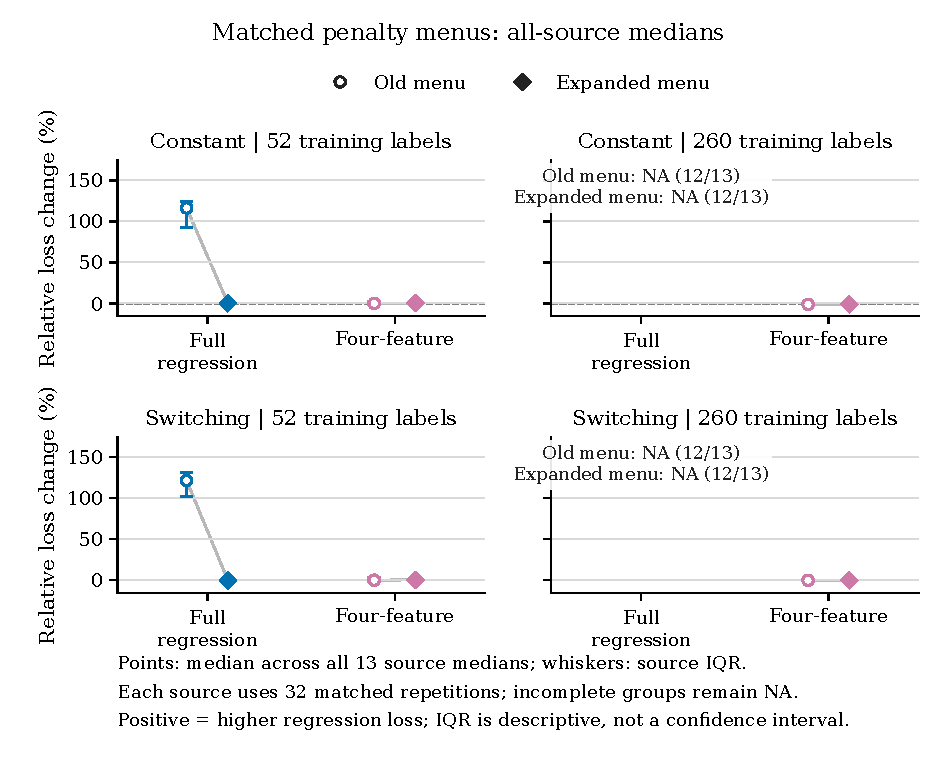
\includegraphics[width=.98\linewidth]{figures/v10-menu-isolation.pdf}
\caption{Paired penalty-menu isolation on unchanged calibrated paths. The expanded menu removes the large short-history full-regression loss in both arms. Longer-history full-regression summaries remain unavailable because a required repetition fails in each arm, with no successful-subset replacement.}\label{fig:mechanism}
\end{figure}

At history 260, one required full-regression repetition fails in each arm under the old low penalty. Both summaries across all thirteen sources remain unavailable. The experiment retains every failed cell and performs no retry. Earlier daily moment-qualification and hourly optimization failures also remain unavailable. Absence of a five-point switching increment is not evidence of equivalence.

The identification qualification above concerns the paired simulated menu intervention. The additional financial finite-menu diagnostic is described in Section~\ref{sup:v12-details}.

\paragraph{Procedure and complete-source inventory.}
Both QR variants use penalties $\{.001,.01,.1,1,10,\infty\}$; the infinite candidate is ordinary intercept-only I, distinct from corrected-rank F. Full regression requires every candidate to complete. Four-feature regression selects from its completed eligible candidates, as before. Exact ties now prefer stronger shrinkage in both variants; no actual exact tie occurred. The switching-phase denominator remains thirty-two. Two pilot repetitions selected the full thirty-two formal repetitions before launch. The simulated feature clock is inherited hourly geometry despite weekly calibration parameters; it is not a literal weekly-calendar replay.

The design preceded every new path calculation. M1 requires the constant-arm history-52 full-regression median within five percent of F. M2 requires the switching median at least five percentage points higher. M3 requires both aggregate improvements and at least twelve jointly improving sources. M1 and M3 hold; M2 fails. Full history-260 regression summaries remain unavailable after the required TIPS-G11 repetition fails in both arms. Successful repetitions or twelve-source subsets never replace them.

\par\smallskip\noindent\begin{minipage}{\linewidth}\footnotesize Constant=C; switching=S. Positive percentages mean higher loss than F. NA retains the whole failed cell; source medians and old results remain separate.\end{minipage}
\begingroup\scriptsize\renewcommand{\arraystretch}{.96}
\begin{longtable}{llrrrrrl}
\caption{Every menu-isolation source/arm/history/method cell. Relative-loss medians use all required repetitions.}\label{tab:v10-menu-full}\\
\toprule Source & Arm & History & Predictors & Original median & Expanded median & Complete/required & State \\\midrule\endfirsthead
\toprule Source & Arm & History & Predictors & Original median & Expanded median & Complete/required & State \\\midrule\endhead
GS-B & C & 52 & 33 & 117.16 & 4.24 & 32/32 & COMPLETE \\
GS-B & C & 52 & 4 & 7.20 & 8.70 & 32/32 & COMPLETE \\
GS-B & C & 260 & 33 & 2.90 & 0.10 & 32/32 & COMPLETE \\
GS-B & C & 260 & 4 & -2.02 & -1.92 & 32/32 & COMPLETE \\
GS-B & S & 52 & 33 & 91.35 & 2.47 & 32/32 & COMPLETE \\
GS-B & S & 52 & 4 & 3.22 & 3.17 & 32/32 & COMPLETE \\
GS-B & S & 260 & 33 & 4.56 & 0.56 & 32/32 & COMPLETE \\
GS-B & S & 260 & 4 & 0.23 & 0.09 & 32/32 & COMPLETE \\
MBS-TOT & C & 52 & 33 & 79.84 & -0.49 & 32/32 & COMPLETE \\
MBS-TOT & C & 52 & 4 & -0.87 & -0.70 & 32/32 & COMPLETE \\
MBS-TOT & C & 260 & 33 & 7.02 & 0.97 & 32/32 & COMPLETE \\
MBS-TOT & C & 260 & 4 & -5.00 & -5.15 & 32/32 & COMPLETE \\
MBS-TOT & S & 52 & 33 & 140.83 & -0.59 & 32/32 & COMPLETE \\
MBS-TOT & S & 52 & 4 & -0.44 & -0.92 & 32/32 & COMPLETE \\
MBS-TOT & S & 260 & 33 & 18.77 & 0.91 & 32/32 & COMPLETE \\
MBS-TOT & S & 260 & 4 & -0.06 & -0.22 & 32/32 & COMPLETE \\
CS-TOT & C & 52 & 33 & 124.34 & -3.01 & 32/32 & COMPLETE \\
CS-TOT & C & 52 & 4 & -3.07 & -3.07 & 32/32 & COMPLETE \\
CS-TOT & C & 260 & 33 & 2.68 & -0.19 & 32/32 & COMPLETE \\
CS-TOT & C & 260 & 4 & -1.21 & -1.13 & 32/32 & COMPLETE \\
CS-TOT & S & 52 & 33 & 124.34 & -3.01 & 32/32 & COMPLETE \\
CS-TOT & S & 52 & 4 & -3.07 & -3.07 & 32/32 & COMPLETE \\
CS-TOT & S & 260 & 33 & 2.68 & -0.19 & 32/32 & COMPLETE \\
CS-TOT & S & 260 & 4 & -1.21 & -1.13 & 32/32 & COMPLETE \\
FGS-TOT & C & 52 & 33 & 201.01 & 4.44 & 32/32 & COMPLETE \\
FGS-TOT & C & 52 & 4 & 1.90 & 1.90 & 32/32 & COMPLETE \\
FGS-TOT & C & 260 & 33 & 13.76 & 1.34 & 32/32 & COMPLETE \\
FGS-TOT & C & 260 & 4 & -2.98 & -2.98 & 32/32 & COMPLETE \\
FGS-TOT & S & 52 & 33 & 170.12 & -0.23 & 32/32 & COMPLETE \\
FGS-TOT & S & 52 & 4 & -4.36 & -4.36 & 32/32 & COMPLETE \\
FGS-TOT & S & 260 & 33 & 15.48 & -0.40 & 32/32 & COMPLETE \\
FGS-TOT & S & 260 & 4 & 0.23 & 0.48 & 32/32 & COMPLETE \\
TIPS-L2 & C & 52 & 33 & 119.29 & -0.54 & 32/32 & COMPLETE \\
TIPS-L2 & C & 52 & 4 & -2.10 & -2.10 & 32/32 & COMPLETE \\
TIPS-L2 & C & 260 & 33 & 9.32 & 0.64 & 32/32 & COMPLETE \\
TIPS-L2 & C & 260 & 4 & -1.69 & -1.69 & 32/32 & COMPLETE \\
TIPS-L2 & S & 52 & 33 & 101.92 & 0.53 & 32/32 & COMPLETE \\
TIPS-L2 & S & 52 & 4 & -0.03 & 0.38 & 32/32 & COMPLETE \\
TIPS-L2 & S & 260 & 33 & 8.88 & -0.38 & 32/32 & COMPLETE \\
TIPS-L2 & S & 260 & 4 & -0.27 & -0.28 & 32/32 & COMPLETE \\
TIPS-G11 & C & 52 & 33 & 131.26 & 0.98 & 32/32 & COMPLETE \\
TIPS-G11 & C & 52 & 4 & 1.11 & 1.14 & 32/32 & COMPLETE \\
TIPS-G11 & C & 260 & 33 & NA & NA & 31/32 & FAILED \\
TIPS-G11 & C & 260 & 4 & -0.48 & -0.49 & 32/32 & COMPLETE \\
TIPS-G11 & S & 52 & 33 & 131.26 & 0.98 & 32/32 & COMPLETE \\
TIPS-G11 & S & 52 & 4 & 1.11 & 1.14 & 32/32 & COMPLETE \\
TIPS-G11 & S & 260 & 33 & NA & NA & 31/32 & FAILED \\
TIPS-G11 & S & 260 & 4 & -0.48 & -0.49 & 32/32 & COMPLETE \\
TIPS-G2 & C & 52 & 33 & 107.85 & -4.00 & 32/32 & COMPLETE \\
TIPS-G2 & C & 52 & 4 & -1.55 & -1.69 & 32/32 & COMPLETE \\
TIPS-G2 & C & 260 & 33 & 13.09 & 0.12 & 32/32 & COMPLETE \\
TIPS-G2 & C & 260 & 4 & -0.29 & -0.43 & 32/32 & COMPLETE \\
TIPS-G2 & S & 52 & 33 & 107.85 & -4.00 & 32/32 & COMPLETE \\
TIPS-G2 & S & 52 & 4 & -1.55 & -1.69 & 32/32 & COMPLETE \\
TIPS-G2 & S & 260 & 33 & 13.09 & 0.12 & 32/32 & COMPLETE \\
TIPS-G2 & S & 260 & 4 & -0.29 & -0.43 & 32/32 & COMPLETE \\
TIPS-G6L11 & C & 52 & 33 & 92.36 & 1.00 & 32/32 & COMPLETE \\
TIPS-G6L11 & C & 52 & 4 & 0.11 & 0.44 & 32/32 & COMPLETE \\
TIPS-G6L11 & C & 260 & 33 & 15.63 & 2.53 & 32/32 & COMPLETE \\
TIPS-G6L11 & C & 260 & 4 & -0.54 & -0.64 & 32/32 & COMPLETE \\
TIPS-G6L11 & S & 52 & 33 & 121.40 & 3.18 & 32/32 & COMPLETE \\
TIPS-G6L11 & S & 52 & 4 & 3.27 & 3.68 & 32/32 & COMPLETE \\
TIPS-G6L11 & S & 260 & 33 & 20.88 & 1.90 & 32/32 & COMPLETE \\
TIPS-G6L11 & S & 260 & 4 & 1.23 & 1.23 & 32/32 & COMPLETE \\
GSC-L2 & C & 52 & 33 & 116.24 & 0.21 & 32/32 & COMPLETE \\
GSC-L2 & C & 52 & 4 & -0.02 & 1.85 & 32/32 & COMPLETE \\
GSC-L2 & C & 260 & 33 & 10.40 & -0.21 & 32/32 & COMPLETE \\
GSC-L2 & C & 260 & 4 & -0.80 & -1.22 & 32/32 & COMPLETE \\
GSC-L2 & S & 52 & 33 & 123.05 & -1.88 & 32/32 & COMPLETE \\
GSC-L2 & S & 52 & 4 & -2.47 & -2.17 & 32/32 & COMPLETE \\
GSC-L2 & S & 260 & 33 & 24.51 & 0.08 & 32/32 & COMPLETE \\
GSC-L2 & S & 260 & 4 & 0.81 & 0.87 & 32/32 & COMPLETE \\
GSC-G2L3 & C & 52 & 33 & 112.85 & 0.74 & 32/32 & COMPLETE \\
GSC-G2L3 & C & 52 & 4 & -0.43 & -0.28 & 32/32 & COMPLETE \\
GSC-G2L3 & C & 260 & 33 & 1.42 & 0.36 & 32/32 & COMPLETE \\
GSC-G2L3 & C & 260 & 4 & -1.39 & -1.02 & 32/32 & COMPLETE \\
GSC-G2L3 & S & 52 & 33 & 109.05 & 0.02 & 32/32 & COMPLETE \\
GSC-G2L3 & S & 52 & 4 & 10.61 & 10.73 & 32/32 & COMPLETE \\
GSC-G2L3 & S & 260 & 33 & -0.63 & -1.22 & 32/32 & COMPLETE \\
GSC-G2L3 & S & 260 & 4 & -3.84 & -3.95 & 32/32 & COMPLETE \\
GSC-G3L6 & C & 52 & 33 & 135.13 & 0.90 & 32/32 & COMPLETE \\
GSC-G3L6 & C & 52 & 4 & 2.78 & 2.43 & 32/32 & COMPLETE \\
GSC-G3L6 & C & 260 & 33 & -1.44 & -1.16 & 32/32 & COMPLETE \\
GSC-G3L6 & C & 260 & 4 & -1.26 & -1.37 & 32/32 & COMPLETE \\
GSC-G3L6 & S & 52 & 33 & 166.48 & 4.12 & 32/32 & COMPLETE \\
GSC-G3L6 & S & 52 & 4 & 5.26 & 6.42 & 32/32 & COMPLETE \\
GSC-G3L6 & S & 260 & 33 & 13.34 & 1.34 & 32/32 & COMPLETE \\
GSC-G3L6 & S & 260 & 4 & 0.31 & 0.61 & 32/32 & COMPLETE \\
GSC-G6L7 & C & 52 & 33 & 90.84 & -0.32 & 32/32 & COMPLETE \\
GSC-G6L7 & C & 52 & 4 & 1.73 & 2.14 & 32/32 & COMPLETE \\
GSC-G6L7 & C & 260 & 33 & 9.12 & 0.02 & 32/32 & COMPLETE \\
GSC-G6L7 & C & 260 & 4 & -0.66 & -0.75 & 32/32 & COMPLETE \\
GSC-G6L7 & S & 52 & 33 & 90.84 & -0.32 & 32/32 & COMPLETE \\
GSC-G6L7 & S & 52 & 4 & 1.73 & 2.14 & 32/32 & COMPLETE \\
GSC-G6L7 & S & 260 & 33 & 9.12 & 0.02 & 32/32 & COMPLETE \\
GSC-G6L7 & S & 260 & 4 & -0.66 & -0.75 & 32/32 & COMPLETE \\
GSC-G7L11 & C & 52 & 33 & 92.90 & -0.52 & 32/32 & COMPLETE \\
GSC-G7L11 & C & 52 & 4 & -4.71 & -4.35 & 32/32 & COMPLETE \\
GSC-G7L11 & C & 260 & 33 & 3.61 & -0.36 & 32/32 & COMPLETE \\
GSC-G7L11 & C & 260 & 4 & -0.51 & -0.55 & 32/32 & COMPLETE \\
GSC-G7L11 & S & 52 & 33 & 80.11 & -2.78 & 32/32 & COMPLETE \\
GSC-G7L11 & S & 52 & 4 & -2.03 & -2.67 & 32/32 & COMPLETE \\
GSC-G7L11 & S & 260 & 33 & -3.41 & 0.20 & 32/32 & COMPLETE \\
GSC-G7L11 & S & 260 & 4 & -5.15 & -5.15 & 32/32 & COMPLETE \\
\bottomrule\end{longtable}\endgroup


\clearpage

\section{CFTC sources, eligibility and information dates}\label{sup:v10-cftc}
The source is the CFTC TFF futures-only historical backcast for 2006--2016 plus annual 2017--2026 files. The retained observations begin in 2010. All eleven original source archives remain public; no other new financial data were acquired.

A complete generated calendar contains 877 Monday-labeled report weeks, from 2010-01-04 through 2026-10-19. Economic position dates are retained separately. A code needs one valid observation per week, a stable exchange and stable contract units. Missing weeks, duplicates and changes disqualify a contract rather than trigger interpolation or splicing. Known consolidation prefixes 13874,20974,12460 are excluded before ranking. This conservative rule is broader than the documented plus-suffixed codes. Full-period mean open interest ranks survivors, with literal-code ties. Seventeen of 141 observed codes qualify; the top-twenty cap never changes that count.
The \href{https://github.com/ByronLi0207/financial-mathematics-paper-20261020/blob/final-jof/results/v10/cftc/eligibility.json}{complete code-level eligibility and exclusions} preserve every screening decision.

Validation indices are 553--604; evaluation indices are 611--870. All labels use horizon six, leaving six unissued origins between the segments. Validation position dates are 2020-08-11--2021-08-03; the last validation label ends 2021-09-14. Evaluation position dates are 2021-09-21--2026-09-08; the last evaluation label ends 2026-10-20. Training labels at refit r span r-H-W+1 through r-H. Monday labels index the inherited feature calendar; they do not claim Monday public availability. Actual positions are normally measured Tuesday and released Friday at 15:30 Eastern. Holiday, shutdown and ION-related publication delays prevent a first-release interpretation.

The selected category series are listed below. Net positions equal dealer long minus short in raw contract counts. Equal-weight median percentage changes preserve within-contract units; they are not common-dollar portfolio risk.
\begin{center}\scriptsize\begin{longtable}{lp{7.1cm}rr}
\toprule Code & Latest contract name & Mean open interest & Weeks \\\midrule\endhead
044601 & UST 5Y NOTE - CHICAGO BOARD OF TRADE & 3479174.2 & 877 \\
043602 & UST 10Y NOTE - CHICAGO BOARD OF TRADE & 3344673.4 & 877 \\
042601 & UST 2Y NOTE - CHICAGO BOARD OF TRADE & 2170647.9 & 877 \\
045601 & FED FUNDS - CHICAGO BOARD OF TRADE & 1282757.7 & 877 \\
020601 & UST BOND - CHICAGO BOARD OF TRADE & 999944.0 & 877 \\
099741 & EURO FX - CHICAGO MERCANTILE EXCHANGE & 503616.5 & 877 \\
1170E1 & VIX FUTURES - CBOE FUTURES EXCHANGE & 356897.7 & 877 \\
097741 & JAPANESE YEN - CHICAGO MERCANTILE EXCHANGE & 210863.1 & 877 \\
096742 & BRITISH POUND - CHICAGO MERCANTILE EXCHANGE & 197853.5 & 877 \\
095741 & MEXICAN PESO - CHICAGO MERCANTILE EXCHANGE & 174995.0 & 877 \\
090741 & CANADIAN DOLLAR - CHICAGO MERCANTILE EXCHANGE & 166229.3 & 877 \\
232741 & AUSTRALIAN DOLLAR - CHICAGO MERCANTILE EXCHANGE & 154802.4 & 877 \\
33874A & E-MINI S\&P 400 STOCK INDEX - CHICAGO MERCANTILE EXCHANGE & 75156.1 & 877 \\
240743 & NIKKEI STOCK AVERAGE YEN DENOM - CHICAGO MERCANTILE EXCHANGE & 59766.6 & 877 \\
092741 & SWISS FRANC - CHICAGO MERCANTILE EXCHANGE & 57197.3 & 877 \\
098662 & USD INDEX - ICE FUTURES U.S. & 52473.9 & 877 \\
112741 & NZ DOLLAR - CHICAGO MERCANTILE EXCHANGE & 44292.0 & 877 \\
\bottomrule\end{longtable}\end{center}

The six methods are corrected-rank F, ordinary I, four- and thirty-three-predictor regression, and finite delayed ACI-style F/QR33. Both regressions use the six-point menu. The paired ACI wrappers retain the existing finite calibration with delayed matured feedback; no asymptotic coverage claim is attached. The original six-procedure, two-history study has 204 complete method cells without a numerical retry. The separate registered extension below adds only the three named procedures at the longer history. The full cell CSV and trace ZIP retain absolute scores, breaches, selected penalties and gamma values.

For the CFTC delayed wrappers, gamma belongs to $\{.001,.005,.01,.05\}$. Completed candidates rank by validation coverage-distance, then pinball loss, then smaller gamma. Initialization requires at least nineteen matured scores. Updates wait for the full six-record label, and evaluation carries the validation state. The six unissued gap origins create no artificial reports or feedback events. These settings accompany histories 52/260, 52 validation origins, 260 evaluation origins and 13-record refits; none is retuned after evaluation.

Two narrow official-format clarifications follow the original design and acquisition but precede every forecast. The first accepts only the official midnight suffix after the date; the second accepts integer counts written with an all-zero decimal suffix. Neither changes a mathematical count, sample threshold, screen or forecast setting. Original failed technical preparation receipts remain visible. This is not a claim of fully observation-blind ingestion design.

\clearpage

\section{Complete model confidence sets}\label{sup:v10-mcs}
The registered ninety-percent MCS uses the range statistic and 1,000 stationary-bootstrap draws, with block length $\max\{H,\lceil n^{1/3}\rceil\}$ in arch 8.0.0. Deterministic source/grid seeds and method order are recorded in the design. Every claimed complete report uses its entire declared origin grid and common target. Missing stored losses are derived only from saved reports, without issuing forecasts or fitting models. Every one of 98 comparisons completes. The 60 known unavailable slots remain unavailable, not statistical exclusions.

Distinct procedure labels retain their classification even when a selected penalty is infinite or reports coincide. Exact duplicate loss columns enter the library once; all associated procedure labels then receive the same p-value and inclusion partition. Conditional slots use their declared procedure identity. Matched F/I membership, literal uniqueness and unique-loss-class membership differ. Across the entire inventory, 90/98 sets contain matched F/I, 2/98 have a sole literal F/I member, and 4/98 have a sole loss class containing F/I. Conditional exclusion is 197/683 complete slots. Related sources and overlapping tasks provide no independent cross-grid test or simultaneous future guarantee.

% Generated by notes/v10/build_mcs_compact.py; display only.
\begingroup
\fontsize{7.1}{8.5}\selectfont
\setlength{\tabcolsep}{1.35pt}
\renewcommand{\arraystretch}{1.06}
\setlength{\LTcapwidth}{\linewidth}
\noindent\textbf{Complete pre-specified MCS membership and p-values.}
All 98 source/period/$H$/$W$ comparisons are retained. Bold p-values denote included procedures using the saved literal rule $p>0.10$; ordinary type denotes exclusion. Values are rounded to three decimals only for display. Membership uses unrounded saved values; exact p-values are public in \texttt{results/v10/mcs/report-values.json}. \textsc{NA} denotes a known unavailable procedure, never a statistical exclusion; --- means that procedure was not pre-specified in that particular grid.
Multi-member exact-loss classes carry a superscript equal to the representative method ID on \emph{every} member, including the representative. Unmarked values are singleton classes. Method IDs are display aliases only; all full labels and classifications appear in the final legend.
The pre-specified procedure uses 1000 stationary-bootstrap replications, confidence 0.90, statistic $R$, and block length $\max\{H,\lceil n^{1/3}\rceil\}$. Analytic identical-loss or single-method cases retain their saved status; no new inference is performed for this table.

\noindent\textbf{FX original.} Each method column is shown once for every row of this group.\par
\begin{longtable}{@{}lrrrrrrrrrrrrrr@{}}
\caption{FX original; method block 1/3. Full-grid $n=6625$.}\\
\toprule
Source & \rotatebox{90}{Horizon} & \rotatebox{90}{History} & \rotatebox{90}{\shortstack[l]{Hist.\\headroom}} & \rotatebox{90}{\shortstack[l]{Intercept\\only}} & \rotatebox{90}{\shortstack[l]{Cal. SAV\\history}} & \rotatebox{90}{\shortstack[l]{Cal. SAV\\regression}} & \rotatebox{90}{\shortstack[l]{SAV\\headroom}} & \rotatebox{90}{\shortstack[l]{Expanded\\full reg.}} & \rotatebox{90}{\shortstack[l]{Endpoint\\plug-in}} & \rotatebox{90}{\shortstack[l]{Four-\\feature}} & \rotatebox{90}{\shortstack[l]{Legacy\\multi-fold}} & \rotatebox{90}{\shortstack[l]{Finite\\ridge}} & \rotatebox{90}{\shortstack[l]{Expanded\\ridge}} & \rotatebox{90}{\shortstack[l]{One-SE\\ridge}} \\
\midrule
\endfirsthead
\toprule
Source & \rotatebox{90}{Horizon} & \rotatebox{90}{History} & \rotatebox{90}{\shortstack[l]{Hist.\\headroom}} & \rotatebox{90}{\shortstack[l]{Intercept\\only}} & \rotatebox{90}{\shortstack[l]{Cal. SAV\\history}} & \rotatebox{90}{\shortstack[l]{Cal. SAV\\regression}} & \rotatebox{90}{\shortstack[l]{SAV\\headroom}} & \rotatebox{90}{\shortstack[l]{Expanded\\full reg.}} & \rotatebox{90}{\shortstack[l]{Endpoint\\plug-in}} & \rotatebox{90}{\shortstack[l]{Four-\\feature}} & \rotatebox{90}{\shortstack[l]{Legacy\\multi-fold}} & \rotatebox{90}{\shortstack[l]{Finite\\ridge}} & \rotatebox{90}{\shortstack[l]{Expanded\\ridge}} & \rotatebox{90}{\shortstack[l]{One-SE\\ridge}} \\
\midrule
\endhead
\midrule\multicolumn{15}{r}{Continued on next page}\\\endfoot
\bottomrule\endlastfoot
fx\_hourly & 6 & 720 & $0.000$ & $0.002^{\mathrm{M02}}$ & $0.000$ & $0.019$ & $0.000$ & $0.040^{\mathrm{M10}}$ & $0.000$ & $0.010$ & \textsc{NA} & $0.040^{\mathrm{M10}}$ & $0.040^{\mathrm{M10}}$ & $0.002^{\mathrm{M02}}$ \\
fx\_hourly & 6 & 2880 & $0.000$ & $0.000^{\mathrm{M02}}$ & $0.000$ & $\mathbf{0.385}$ & $0.000$ & $\mathbf{1.000}^{\mathrm{M10}}$ & $0.000$ & $0.001$ & --- & $\mathbf{1.000}^{\mathrm{M10}}$ & $\mathbf{1.000}^{\mathrm{M10}}$ & $0.000^{\mathrm{M02}}$ \\
fx\_hourly & 24 & 720 & $\mathbf{0.696}$ & $\mathbf{0.760}\hphantom{^{\mathrm{M00}}}$ & $0.009$ & $0.000$ & $\mathbf{0.792}$ & $0.009^{\mathrm{M10}}$ & $0.011$ & $\mathbf{0.250}$ & \textsc{NA} & $0.009^{\mathrm{M10}}$ & $0.009^{\mathrm{M10}}$ & $0.009^{\mathrm{M10}}$ \\
fx\_hourly & 24 & 2880 & $\mathbf{0.360}$ & $\mathbf{0.360}\hphantom{^{\mathrm{M00}}}$ & $\mathbf{0.360}$ & $\mathbf{0.360}$ & $\mathbf{0.360}$ & $\mathbf{0.360}^{\mathrm{M10}}$ & $0.005$ & $\mathbf{0.360}$ & --- & $\mathbf{0.360}^{\mathrm{M10}}$ & $\mathbf{0.360}^{\mathrm{M10}}$ & $0.078^{\mathrm{M16}}$ \\
\end{longtable}

\begin{longtable}{@{}lrrrrrrrrrrrrrr@{}}
\caption{FX original; method block 2/3. Full-grid $n=6625$.}\\
\toprule
Source & \rotatebox{90}{Horizon} & \rotatebox{90}{History} & \rotatebox{90}{\shortstack[l]{Multi-fold\\one-SE}} & \rotatebox{90}{\shortstack[l]{Filtered\\paths}} & \rotatebox{90}{\shortstack[l]{Peak-tail\\fit}} & \rotatebox{90}{\shortstack[l]{Quantile\\forest}} & \rotatebox{90}{\shortstack[l]{Nearest\\states}} & \rotatebox{90}{\shortstack[l]{Original\\full reg.}} & \rotatebox{90}{\shortstack[l]{Scaled\\neighbors}} & \rotatebox{90}{\shortstack[l]{Fixed\\peak}} & \rotatebox{90}{\shortstack[l]{Fixed\\transl.}} & \rotatebox{90}{\shortstack[l]{State\\headroom}} & \rotatebox{90}{\shortstack[l]{State\\peak}} & \rotatebox{90}{\shortstack[l]{State\\transl.}} \\
\midrule
\endfirsthead
\toprule
Source & \rotatebox{90}{Horizon} & \rotatebox{90}{History} & \rotatebox{90}{\shortstack[l]{Multi-fold\\one-SE}} & \rotatebox{90}{\shortstack[l]{Filtered\\paths}} & \rotatebox{90}{\shortstack[l]{Peak-tail\\fit}} & \rotatebox{90}{\shortstack[l]{Quantile\\forest}} & \rotatebox{90}{\shortstack[l]{Nearest\\states}} & \rotatebox{90}{\shortstack[l]{Original\\full reg.}} & \rotatebox{90}{\shortstack[l]{Scaled\\neighbors}} & \rotatebox{90}{\shortstack[l]{Fixed\\peak}} & \rotatebox{90}{\shortstack[l]{Fixed\\transl.}} & \rotatebox{90}{\shortstack[l]{State\\headroom}} & \rotatebox{90}{\shortstack[l]{State\\peak}} & \rotatebox{90}{\shortstack[l]{State\\transl.}} \\
\midrule
\endhead
\midrule\multicolumn{15}{r}{Continued on next page}\\\endfoot
\bottomrule\endlastfoot
fx\_hourly & 6 & 720 & --- & \textsc{NA} & \textsc{NA} & $0.002$ & $0.014$ & $0.040^{\mathrm{M10}}$ & $0.016$ & $0.000$ & $0.004$ & $0.002$ & $0.000$ & $0.014$ \\
fx\_hourly & 6 & 2880 & $\mathbf{1.000}^{\mathrm{M10}}$ & $0.000$ & $0.000$ & $0.001$ & $0.054$ & $\mathbf{1.000}^{\mathrm{M10}}$ & $0.039$ & $0.000$ & $0.000$ & --- & --- & --- \\
fx\_hourly & 24 & 720 & --- & \textsc{NA} & \textsc{NA} & $\mathbf{0.199}$ & $\mathbf{0.445}$ & $0.009^{\mathrm{M10}}$ & $\mathbf{0.347}$ & $0.000$ & $\mathbf{0.696}$ & $\mathbf{0.792}$ & $0.067$ & $\mathbf{0.792}$ \\
fx\_hourly & 24 & 2880 & $0.078^{\mathrm{M16}}$ & $0.079$ & $0.002$ & $\mathbf{0.153}$ & $0.078$ & $\mathbf{0.360}^{\mathrm{M10}}$ & $0.052$ & $0.000$ & $\mathbf{0.360}$ & --- & --- & --- \\
\end{longtable}

\begin{longtable}{@{}lrrrrrrr@{}}
\caption{FX original; method block 3/3. Full-grid $n=6625$.}\\
\toprule
Source & \rotatebox{90}{Horizon} & \rotatebox{90}{History} & \rotatebox{90}{\shortstack[l]{Rolling\\headroom}} & \rotatebox{90}{\shortstack[l]{Rolling\\peak}} & \rotatebox{90}{\shortstack[l]{Rolling\\transl.}} & \rotatebox{90}{\shortstack[l]{Mean\\combination}} & \rotatebox{90}{\shortstack[l]{Median\\combination}} \\
\midrule
\endfirsthead
\toprule
Source & \rotatebox{90}{Horizon} & \rotatebox{90}{History} & \rotatebox{90}{\shortstack[l]{Rolling\\headroom}} & \rotatebox{90}{\shortstack[l]{Rolling\\peak}} & \rotatebox{90}{\shortstack[l]{Rolling\\transl.}} & \rotatebox{90}{\shortstack[l]{Mean\\combination}} & \rotatebox{90}{\shortstack[l]{Median\\combination}} \\
\midrule
\endhead
\midrule\multicolumn{8}{r}{Continued on next page}\\\endfoot
\bottomrule\endlastfoot
fx\_hourly & 6 & 720 & $0.002$ & $0.000$ & $0.003$ & $\mathbf{1.000}$ & $0.047$ \\
fx\_hourly & 6 & 2880 & $0.000$ & $0.000$ & $0.000$ & $0.039$ & $0.057$ \\
fx\_hourly & 24 & 720 & $\mathbf{0.792}$ & $0.000$ & $\mathbf{1.000}$ & $\mathbf{0.696}$ & $\mathbf{0.551}$ \\
fx\_hourly & 24 & 2880 & $\mathbf{0.360}$ & $0.000$ & $\mathbf{0.360}$ & $\mathbf{1.000}$ & $\mathbf{0.360}$ \\
\end{longtable}

\clearpage
\noindent\textbf{FX early 2015.} Each method column is shown once for every row of this group.\par
\begin{longtable}{@{}lrrrrrrrrrrr@{}}
\caption{FX early 2015; method block 1/1. Full-grid $n=1440$.}\\
\toprule
Source & \rotatebox{90}{Horizon} & \rotatebox{90}{History} & \rotatebox{90}{\shortstack[l]{Hist.\\headroom}} & \rotatebox{90}{\shortstack[l]{Intercept\\only}} & \rotatebox{90}{\shortstack[l]{Legacy\\multi-fold}} & \rotatebox{90}{\shortstack[l]{Finite\\ridge}} & \rotatebox{90}{\shortstack[l]{Expanded\\ridge}} & \rotatebox{90}{\shortstack[l]{One-SE\\ridge}} & \rotatebox{90}{\shortstack[l]{Multi-fold\\one-SE}} & \rotatebox{90}{\shortstack[l]{Original\\full reg.}} & \rotatebox{90}{\shortstack[l]{Original\\roll. hist.}} \\
\midrule
\endfirsthead
\toprule
Source & \rotatebox{90}{Horizon} & \rotatebox{90}{History} & \rotatebox{90}{\shortstack[l]{Hist.\\headroom}} & \rotatebox{90}{\shortstack[l]{Intercept\\only}} & \rotatebox{90}{\shortstack[l]{Legacy\\multi-fold}} & \rotatebox{90}{\shortstack[l]{Finite\\ridge}} & \rotatebox{90}{\shortstack[l]{Expanded\\ridge}} & \rotatebox{90}{\shortstack[l]{One-SE\\ridge}} & \rotatebox{90}{\shortstack[l]{Multi-fold\\one-SE}} & \rotatebox{90}{\shortstack[l]{Original\\full reg.}} & \rotatebox{90}{\shortstack[l]{Original\\roll. hist.}} \\
\midrule
\endhead
\midrule\multicolumn{12}{r}{Continued on next page}\\\endfoot
\bottomrule\endlastfoot
fx\_hourly & 6 & 720 & $0.063$ & $\mathbf{0.675}$ & \textsc{NA} & $\mathbf{0.675}^{\mathrm{M14}}$ & $\mathbf{0.675}^{\mathrm{M14}}$ & $\mathbf{0.628}\hphantom{^{\mathrm{M00}}}$ & --- & --- & $\mathbf{1.000}$ \\
fx\_hourly & 6 & 2880 & $0.000$ & $0.000$ & --- & $\mathbf{1.000}^{\mathrm{M14}}$ & $\mathbf{1.000}^{\mathrm{M14}}$ & $0.009\hphantom{^{\mathrm{M00}}}$ & $\mathbf{1.000}^{\mathrm{M14}}$ & $\mathbf{1.000}^{\mathrm{M14}}$ & --- \\
fx\_hourly & 24 & 720 & $0.014$ & $\mathbf{0.242}$ & \textsc{NA} & $\mathbf{1.000}^{\mathrm{M14}}$ & $\mathbf{1.000}^{\mathrm{M14}}$ & $\mathbf{1.000}^{\mathrm{M14}}$ & --- & --- & --- \\
fx\_hourly & 24 & 2880 & $0.000$ & $\mathbf{0.910}$ & --- & $\mathbf{1.000}^{\mathrm{M14}}$ & $\mathbf{1.000}^{\mathrm{M14}}$ & $\mathbf{0.991}^{\mathrm{M16}}$ & $\mathbf{0.991}^{\mathrm{M16}}$ & --- & --- \\
\end{longtable}

\clearpage
\noindent\textbf{Treasury bills.} Each method column is shown once for every row of this group.\par
\begin{longtable}{@{}lrrrrrrrrrrrrrr@{}}
\caption{Treasury bills; method block 1/3. Full-grid $n=277$.}\\
\toprule
Source & \rotatebox{90}{Horizon} & \rotatebox{90}{History} & \rotatebox{90}{\shortstack[l]{Hist.\\headroom}} & \rotatebox{90}{\shortstack[l]{Intercept\\only}} & \rotatebox{90}{\shortstack[l]{Cal. SAV\\history}} & \rotatebox{90}{\shortstack[l]{Cal. SAV\\regression}} & \rotatebox{90}{\shortstack[l]{SAV\\headroom}} & \rotatebox{90}{\shortstack[l]{Expanded\\full reg.}} & \rotatebox{90}{\shortstack[l]{Endpoint\\plug-in}} & \rotatebox{90}{\shortstack[l]{Four-\\feature}} & \rotatebox{90}{\shortstack[l]{Finite\\ridge}} & \rotatebox{90}{\shortstack[l]{Expanded\\ridge}} & \rotatebox{90}{\shortstack[l]{One-SE\\ridge}} & \rotatebox{90}{\shortstack[l]{Multi-fold\\one-SE}} \\
\midrule
\endfirsthead
\toprule
Source & \rotatebox{90}{Horizon} & \rotatebox{90}{History} & \rotatebox{90}{\shortstack[l]{Hist.\\headroom}} & \rotatebox{90}{\shortstack[l]{Intercept\\only}} & \rotatebox{90}{\shortstack[l]{Cal. SAV\\history}} & \rotatebox{90}{\shortstack[l]{Cal. SAV\\regression}} & \rotatebox{90}{\shortstack[l]{SAV\\headroom}} & \rotatebox{90}{\shortstack[l]{Expanded\\full reg.}} & \rotatebox{90}{\shortstack[l]{Endpoint\\plug-in}} & \rotatebox{90}{\shortstack[l]{Four-\\feature}} & \rotatebox{90}{\shortstack[l]{Finite\\ridge}} & \rotatebox{90}{\shortstack[l]{Expanded\\ridge}} & \rotatebox{90}{\shortstack[l]{One-SE\\ridge}} & \rotatebox{90}{\shortstack[l]{Multi-fold\\one-SE}} \\
\midrule
\endhead
\midrule\multicolumn{15}{r}{Continued on next page}\\\endfoot
\bottomrule\endlastfoot
nyfed\_weekly & 6 & 52 & $\mathbf{0.809}^{\mathrm{M01}}$ & $\mathbf{0.400}^{\mathrm{M02}}$ & $0.000$ & $0.004$ & $0.045$ & $\mathbf{0.940}^{\mathrm{M10}}$ & $\mathbf{0.810}$ & $\mathbf{0.770}$ & $\mathbf{0.940}^{\mathrm{M10}}$ & $\mathbf{0.400}^{\mathrm{M02}}$ & $\mathbf{0.400}^{\mathrm{M02}}$ & $\mathbf{0.400}^{\mathrm{M02}}$ \\
nyfed\_weekly & 6 & 260 & $\mathbf{0.663}\hphantom{^{\mathrm{M00}}}$ & $0.073\hphantom{^{\mathrm{M00}}}$ & $\mathbf{0.144}$ & $\mathbf{0.194}$ & $\mathbf{0.273}$ & $\mathbf{0.452}^{\mathrm{M10}}$ & $\mathbf{0.982}$ & $\mathbf{0.622}$ & $\mathbf{0.452}^{\mathrm{M10}}$ & $\mathbf{0.452}^{\mathrm{M10}}$ & $\mathbf{0.622}^{\mathrm{M16}}$ & $\mathbf{0.622}^{\mathrm{M16}}$ \\
nyfed\_weekly & 24 & 52 & $\mathbf{0.862}^{\mathrm{M01}}$ & $\mathbf{0.626}^{\mathrm{M02}}$ & $\mathbf{0.926}$ & $0.004$ & $\mathbf{0.253}$ & $\mathbf{0.925}^{\mathrm{M10}}$ & $\mathbf{0.211}$ & $\mathbf{0.150}$ & $\mathbf{0.925}^{\mathrm{M10}}$ & $\mathbf{0.626}^{\mathrm{M02}}$ & $\mathbf{0.626}^{\mathrm{M02}}$ & $\mathbf{0.626}^{\mathrm{M02}}$ \\
nyfed\_weekly & 24 & 260 & $0.066\hphantom{^{\mathrm{M00}}}$ & $\mathbf{0.165}^{\mathrm{M02}}$ & \textsc{NA} & \textsc{NA} & $\mathbf{0.261}$ & $\mathbf{0.186}^{\mathrm{M10}}$ & $\mathbf{0.186}$ & $\mathbf{0.178}$ & $\mathbf{0.186}^{\mathrm{M10}}$ & $\mathbf{0.186}^{\mathrm{M10}}$ & $\mathbf{0.165}^{\mathrm{M02}}$ & $\mathbf{0.165}^{\mathrm{M02}}$ \\
\end{longtable}

\begin{longtable}{@{}lrrrrrrrrrrrrrr@{}}
\caption{Treasury bills; method block 2/3. Full-grid $n=277$.}\\
\toprule
Source & \rotatebox{90}{Horizon} & \rotatebox{90}{History} & \rotatebox{90}{\shortstack[l]{Filtered\\paths}} & \rotatebox{90}{\shortstack[l]{Peak-tail\\fit}} & \rotatebox{90}{\shortstack[l]{Quantile\\forest}} & \rotatebox{90}{\shortstack[l]{Nearest\\states}} & \rotatebox{90}{\shortstack[l]{Original\\full reg.}} & \rotatebox{90}{\shortstack[l]{Scaled\\neighbors}} & \rotatebox{90}{\shortstack[l]{Fixed\\peak}} & \rotatebox{90}{\shortstack[l]{Fixed\\transl.}} & \rotatebox{90}{\shortstack[l]{State\\headroom}} & \rotatebox{90}{\shortstack[l]{State\\peak}} & \rotatebox{90}{\shortstack[l]{State\\transl.}} & \rotatebox{90}{\shortstack[l]{Rolling\\headroom}} \\
\midrule
\endfirsthead
\toprule
Source & \rotatebox{90}{Horizon} & \rotatebox{90}{History} & \rotatebox{90}{\shortstack[l]{Filtered\\paths}} & \rotatebox{90}{\shortstack[l]{Peak-tail\\fit}} & \rotatebox{90}{\shortstack[l]{Quantile\\forest}} & \rotatebox{90}{\shortstack[l]{Nearest\\states}} & \rotatebox{90}{\shortstack[l]{Original\\full reg.}} & \rotatebox{90}{\shortstack[l]{Scaled\\neighbors}} & \rotatebox{90}{\shortstack[l]{Fixed\\peak}} & \rotatebox{90}{\shortstack[l]{Fixed\\transl.}} & \rotatebox{90}{\shortstack[l]{State\\headroom}} & \rotatebox{90}{\shortstack[l]{State\\peak}} & \rotatebox{90}{\shortstack[l]{State\\transl.}} & \rotatebox{90}{\shortstack[l]{Rolling\\headroom}} \\
\midrule
\endhead
\midrule\multicolumn{15}{r}{Continued on next page}\\\endfoot
\bottomrule\endlastfoot
nyfed\_weekly & 6 & 52 & $\mathbf{0.940}$ & \textsc{NA} & $\mathbf{0.940}$ & $\mathbf{0.809}^{\mathrm{M01}}$ & $0.012$ & $0.016$ & $\mathbf{0.743}$ & $\mathbf{0.767}$ & $\mathbf{0.863}$ & $\mathbf{0.940}$ & $\mathbf{0.802}$ & $\mathbf{0.597}$ \\
nyfed\_weekly & 6 & 260 & $\mathbf{0.897}$ & $\mathbf{0.982}$ & $\mathbf{0.622}$ & $\mathbf{0.845}\hphantom{^{\mathrm{M00}}}$ & $0.028$ & $\mathbf{0.157}$ & $\mathbf{0.982}$ & $\mathbf{0.687}$ & $\mathbf{0.957}$ & $\mathbf{0.982}$ & $\mathbf{0.913}$ & $\mathbf{0.633}$ \\
nyfed\_weekly & 24 & 52 & $\mathbf{0.150}$ & \textsc{NA} & $\mathbf{0.977}$ & $\mathbf{0.862}^{\mathrm{M01}}$ & $\mathbf{0.211}$ & $0.025$ & $\mathbf{0.925}$ & $\mathbf{0.979}$ & $\mathbf{0.862}$ & $\mathbf{0.926}$ & $\mathbf{0.977}$ & $\mathbf{0.925}$ \\
nyfed\_weekly & 24 & 260 & $0.000$ & $0.000$ & $0.066$ & $\mathbf{0.261}\hphantom{^{\mathrm{M00}}}$ & $\mathbf{0.201}$ & $0.000$ & $\mathbf{0.487}$ & $0.072$ & $\mathbf{1.000}$ & $\mathbf{0.336}$ & $\mathbf{0.487}$ & $0.066$ \\
\end{longtable}

\begin{longtable}{@{}lrrrrrr@{}}
\caption{Treasury bills; method block 3/3. Full-grid $n=277$.}\\
\toprule
Source & \rotatebox{90}{Horizon} & \rotatebox{90}{History} & \rotatebox{90}{\shortstack[l]{Rolling\\peak}} & \rotatebox{90}{\shortstack[l]{Rolling\\transl.}} & \rotatebox{90}{\shortstack[l]{Mean\\combination}} & \rotatebox{90}{\shortstack[l]{Median\\combination}} \\
\midrule
\endfirsthead
\toprule
Source & \rotatebox{90}{Horizon} & \rotatebox{90}{History} & \rotatebox{90}{\shortstack[l]{Rolling\\peak}} & \rotatebox{90}{\shortstack[l]{Rolling\\transl.}} & \rotatebox{90}{\shortstack[l]{Mean\\combination}} & \rotatebox{90}{\shortstack[l]{Median\\combination}} \\
\midrule
\endhead
\midrule\multicolumn{7}{r}{Continued on next page}\\\endfoot
\bottomrule\endlastfoot
nyfed\_weekly & 6 & 52 & $\mathbf{1.000}$ & $\mathbf{0.516}$ & $\mathbf{0.940}$ & $\mathbf{0.809}^{\mathrm{M01}}$ \\
nyfed\_weekly & 6 & 260 & $\mathbf{1.000}$ & $\mathbf{0.663}$ & $\mathbf{0.622}$ & $\mathbf{0.848}\hphantom{^{\mathrm{M00}}}$ \\
nyfed\_weekly & 24 & 52 & $\mathbf{0.926}$ & $\mathbf{1.000}$ & $\mathbf{0.925}$ & $\mathbf{0.862}^{\mathrm{M01}}$ \\
nyfed\_weekly & 24 & 260 & $\mathbf{0.624}$ & $0.066$ & $\mathbf{0.336}$ & $\mathbf{0.321}\hphantom{^{\mathrm{M00}}}$ \\
\end{longtable}

\clearpage
\noindent\textbf{Other NYFed panels.} Each method column is shown once for every row of this group.\par
\begin{longtable}{@{}lrrrrrrrrrrrrrr@{}}
\caption{Other NYFed panels; method block 1/1. Full-grid $n=277$.}\\
\toprule
Source & \rotatebox{90}{Horizon} & \rotatebox{90}{History} & \rotatebox{90}{\shortstack[l]{Hist.\\headroom}} & \rotatebox{90}{\shortstack[l]{Intercept\\only}} & \rotatebox{90}{\shortstack[l]{Finite\\ridge}} & \rotatebox{90}{\shortstack[l]{Expanded\\ridge}} & \rotatebox{90}{\shortstack[l]{One-SE\\ridge}} & \rotatebox{90}{\shortstack[l]{Multi-fold\\one-SE}} & \rotatebox{90}{\shortstack[l]{Expanded\\full reg.}} & \rotatebox{90}{\shortstack[l]{Four-\\feature}} & \rotatebox{90}{\shortstack[l]{Endpoint\\plug-in}} & \rotatebox{90}{\shortstack[l]{Original\\full reg.}} & \rotatebox{90}{\shortstack[l]{Mean\\combination}} & \rotatebox{90}{\shortstack[l]{Median\\combination}} \\
\midrule
\endfirsthead
\toprule
Source & \rotatebox{90}{Horizon} & \rotatebox{90}{History} & \rotatebox{90}{\shortstack[l]{Hist.\\headroom}} & \rotatebox{90}{\shortstack[l]{Intercept\\only}} & \rotatebox{90}{\shortstack[l]{Finite\\ridge}} & \rotatebox{90}{\shortstack[l]{Expanded\\ridge}} & \rotatebox{90}{\shortstack[l]{One-SE\\ridge}} & \rotatebox{90}{\shortstack[l]{Multi-fold\\one-SE}} & \rotatebox{90}{\shortstack[l]{Expanded\\full reg.}} & \rotatebox{90}{\shortstack[l]{Four-\\feature}} & \rotatebox{90}{\shortstack[l]{Endpoint\\plug-in}} & \rotatebox{90}{\shortstack[l]{Original\\full reg.}} & \rotatebox{90}{\shortstack[l]{Mean\\combination}} & \rotatebox{90}{\shortstack[l]{Median\\combination}} \\
\midrule
\endhead
\midrule\multicolumn{15}{r}{Continued on next page}\\\endfoot
\bottomrule\endlastfoot
PDPOSCS-TOT & 6 & 52 & $\mathbf{0.312}$ & $\mathbf{1.000}^{\mathrm{M02}}$ & $\mathbf{0.312}^{\mathrm{M14}}$ & $\mathbf{1.000}^{\mathrm{M02}}$ & $\mathbf{1.000}^{\mathrm{M02}}$ & $\mathbf{1.000}^{\mathrm{M02}}$ & $\mathbf{0.312}^{\mathrm{M14}}$ & $\mathbf{0.312}$ & $\mathbf{0.172}$ & $0.095\hphantom{^{\mathrm{M00}}}$ & $\mathbf{0.312}$ & \textsc{NA} \\
PDPOSCS-TOT & 6 & 260 & $\mathbf{0.582}$ & $\mathbf{0.780}^{\mathrm{M02}}$ & $\mathbf{0.243}^{\mathrm{M14}}$ & $\mathbf{0.243}^{\mathrm{M14}}$ & $\mathbf{0.780}^{\mathrm{M02}}$ & $\mathbf{0.780}^{\mathrm{M02}}$ & $\mathbf{0.243}^{\mathrm{M14}}$ & $\mathbf{0.780}$ & $0.000$ & $\mathbf{0.697}\hphantom{^{\mathrm{M00}}}$ & $\mathbf{1.000}$ & \textsc{NA} \\
PDPOSCS-TOT & 24 & 52 & $\mathbf{0.898}$ & $\mathbf{0.898}^{\mathrm{M02}}$ & $\mathbf{0.780}^{\mathrm{M14}}$ & $\mathbf{0.898}^{\mathrm{M02}}$ & $\mathbf{0.898}^{\mathrm{M02}}$ & $\mathbf{0.898}^{\mathrm{M02}}$ & $\mathbf{0.780}^{\mathrm{M14}}$ & $\mathbf{0.898}$ & $\mathbf{1.000}$ & $0.085\hphantom{^{\mathrm{M00}}}$ & $\mathbf{0.780}$ & \textsc{NA} \\
PDPOSCS-TOT & 24 & 260 & $0.000$ & $\mathbf{1.000}^{\mathrm{M02}}$ & $0.010^{\mathrm{M14}}$ & $\mathbf{1.000}^{\mathrm{M02}}$ & $\mathbf{1.000}^{\mathrm{M02}}$ & $\mathbf{1.000}^{\mathrm{M02}}$ & $0.010^{\mathrm{M14}}$ & $0.000$ & $0.000$ & $0.003\hphantom{^{\mathrm{M00}}}$ & $0.000$ & \textsc{NA} \\
PDPOSFGS-TOT & 6 & 52 & $\mathbf{0.248}$ & $\mathbf{1.000}^{\mathrm{M02}}$ & $\mathbf{0.868}^{\mathrm{M14}}$ & $\mathbf{1.000}^{\mathrm{M02}}$ & $\mathbf{1.000}^{\mathrm{M02}}$ & $\mathbf{1.000}^{\mathrm{M02}}$ & $\mathbf{0.868}^{\mathrm{M14}}$ & $\mathbf{0.968}$ & $\mathbf{0.974}$ & $0.014\hphantom{^{\mathrm{M00}}}$ & $\mathbf{0.492}$ & \textsc{NA} \\
PDPOSFGS-TOT & 6 & 260 & $0.017$ & $0.039\hphantom{^{\mathrm{M00}}}$ & $\mathbf{1.000}^{\mathrm{M14}}$ & $\mathbf{1.000}^{\mathrm{M14}}$ & $\mathbf{1.000}^{\mathrm{M14}}$ & $\mathbf{1.000}^{\mathrm{M14}}$ & $\mathbf{1.000}^{\mathrm{M14}}$ & $0.001$ & $0.000$ & $\mathbf{0.709}\hphantom{^{\mathrm{M00}}}$ & $\mathbf{0.709}$ & \textsc{NA} \\
PDPOSFGS-TOT & 24 & 52 & $\mathbf{0.521}$ & $\mathbf{0.390}^{\mathrm{M02}}$ & $\mathbf{0.307}^{\mathrm{M14}}$ & $\mathbf{0.307}^{\mathrm{M14}}$ & $\mathbf{0.390}^{\mathrm{M02}}$ & $\mathbf{0.390}^{\mathrm{M02}}$ & $\mathbf{0.307}^{\mathrm{M14}}$ & $\mathbf{0.521}$ & $\mathbf{1.000}$ & $\mathbf{0.133}\hphantom{^{\mathrm{M00}}}$ & $\mathbf{0.390}$ & \textsc{NA} \\
PDPOSFGS-TOT & 24 & 260 & $0.010$ & $\mathbf{0.772}\hphantom{^{\mathrm{M00}}}$ & $\mathbf{0.772}^{\mathrm{M14}}$ & $\mathbf{0.772}^{\mathrm{M14}}$ & $\mathbf{0.772}^{\mathrm{M14}}$ & $\mathbf{0.772}^{\mathrm{M14}}$ & $\mathbf{0.772}^{\mathrm{M14}}$ & $0.000$ & $\mathbf{1.000}$ & $\mathbf{0.470}\hphantom{^{\mathrm{M00}}}$ & $\mathbf{0.425}$ & \textsc{NA} \\
PDPOSGSC-G2L3 & 6 & 52 & $\mathbf{1.000}$ & $\mathbf{0.208}\hphantom{^{\mathrm{M00}}}$ & $\mathbf{0.189}^{\mathrm{M14}}$ & $\mathbf{0.189}^{\mathrm{M14}}$ & $\mathbf{0.189}^{\mathrm{M14}}$ & $\mathbf{0.189}^{\mathrm{M14}}$ & $\mathbf{0.189}^{\mathrm{M14}}$ & $0.019$ & $0.035$ & $0.018\hphantom{^{\mathrm{M00}}}$ & $\mathbf{0.189}$ & \textsc{NA} \\
PDPOSGSC-G2L3 & 6 & 260 & $\mathbf{0.676}$ & $\mathbf{0.676}\hphantom{^{\mathrm{M00}}}$ & $\mathbf{0.118}^{\mathrm{M14}}$ & $\mathbf{0.118}^{\mathrm{M14}}$ & $\mathbf{0.676}^{\mathrm{M16}}$ & $\mathbf{0.676}^{\mathrm{M16}}$ & $\mathbf{0.118}^{\mathrm{M14}}$ & $\mathbf{0.348}$ & $\mathbf{1.000}$ & $\mathbf{0.118}^{\mathrm{M14}}$ & $\mathbf{0.521}$ & \textsc{NA} \\
PDPOSGSC-G2L3 & 24 & 52 & $\mathbf{1.000}$ & $\mathbf{0.280}^{\mathrm{M02}}$ & $0.004^{\mathrm{M14}}$ & $0.004^{\mathrm{M14}}$ & $0.069\hphantom{^{\mathrm{M00}}}$ & $\mathbf{0.280}^{\mathrm{M02}}$ & $0.004^{\mathrm{M14}}$ & $0.005$ & $0.065$ & $0.004^{\mathrm{M14}}$ & $0.069$ & \textsc{NA} \\
PDPOSGSC-G2L3 & 24 & 260 & $\mathbf{0.204}$ & $\mathbf{0.204}^{\mathrm{M02}}$ & $\mathbf{0.271}^{\mathrm{M14}}$ & $\mathbf{0.204}^{\mathrm{M02}}$ & $\mathbf{0.204}^{\mathrm{M02}}$ & $\mathbf{0.204}^{\mathrm{M02}}$ & $\mathbf{0.271}^{\mathrm{M14}}$ & $\mathbf{0.204}$ & $\mathbf{1.000}$ & $\mathbf{0.245}\hphantom{^{\mathrm{M00}}}$ & $\mathbf{0.271}$ & \textsc{NA} \\
PDPOSGSC-G3L6 & 6 & 52 & $\mathbf{0.624}$ & $\mathbf{0.921}\hphantom{^{\mathrm{M00}}}$ & $\mathbf{0.426}^{\mathrm{M14}}$ & $\mathbf{0.426}^{\mathrm{M14}}$ & $\mathbf{0.602}^{\mathrm{M16}}$ & $\mathbf{0.602}^{\mathrm{M16}}$ & $\mathbf{0.426}^{\mathrm{M14}}$ & $0.033$ & $0.078$ & $0.025\hphantom{^{\mathrm{M00}}}$ & $\mathbf{1.000}$ & \textsc{NA} \\
PDPOSGSC-G3L6 & 6 & 260 & $\mathbf{0.746}$ & $\mathbf{0.437}^{\mathrm{M02}}$ & $\mathbf{0.710}^{\mathrm{M14}}$ & $\mathbf{0.710}^{\mathrm{M14}}$ & $\mathbf{0.437}^{\mathrm{M02}}$ & $\mathbf{0.437}^{\mathrm{M02}}$ & $\mathbf{0.710}^{\mathrm{M14}}$ & $\mathbf{0.437}$ & $\mathbf{0.461}$ & $\mathbf{0.710}^{\mathrm{M14}}$ & $\mathbf{1.000}$ & \textsc{NA} \\
PDPOSGSC-G3L6 & 24 & 52 & $\mathbf{0.471}$ & $\mathbf{0.471}^{\mathrm{M02}}$ & $\mathbf{0.460}^{\mathrm{M14}}$ & $\mathbf{0.460}^{\mathrm{M14}}$ & $\mathbf{0.460}^{\mathrm{M14}}$ & $\mathbf{0.471}^{\mathrm{M02}}$ & $\mathbf{0.460}^{\mathrm{M14}}$ & $0.039$ & $\mathbf{1.000}$ & $0.009\hphantom{^{\mathrm{M00}}}$ & $0.039$ & \textsc{NA} \\
PDPOSGSC-G3L6 & 24 & 260 & $\mathbf{0.103}$ & $\mathbf{0.127}\hphantom{^{\mathrm{M00}}}$ & $\mathbf{1.000}^{\mathrm{M14}}$ & $\mathbf{1.000}^{\mathrm{M14}}$ & $\mathbf{1.000}^{\mathrm{M14}}$ & $\mathbf{1.000}^{\mathrm{M14}}$ & $\mathbf{1.000}^{\mathrm{M14}}$ & $\mathbf{0.103}$ & $\mathbf{0.997}$ & $\mathbf{0.678}\hphantom{^{\mathrm{M00}}}$ & $\mathbf{0.703}$ & \textsc{NA} \\
PDPOSGSC-G6L7 & 6 & 52 & $\mathbf{0.962}$ & $\mathbf{1.000}^{\mathrm{M02}}$ & $\mathbf{0.119}^{\mathrm{M14}}$ & $\mathbf{0.119}^{\mathrm{M14}}$ & $\mathbf{1.000}^{\mathrm{M02}}$ & $\mathbf{1.000}^{\mathrm{M02}}$ & $\mathbf{0.119}^{\mathrm{M14}}$ & $\mathbf{0.119}$ & $\mathbf{0.962}$ & $0.000\hphantom{^{\mathrm{M00}}}$ & $\mathbf{0.258}$ & \textsc{NA} \\
PDPOSGSC-G6L7 & 6 & 260 & $\mathbf{0.366}$ & $\mathbf{0.366}\hphantom{^{\mathrm{M00}}}$ & $0.089^{\mathrm{M14}}$ & $0.089^{\mathrm{M14}}$ & $0.089^{\mathrm{M14}}$ & $0.089^{\mathrm{M14}}$ & $0.089^{\mathrm{M14}}$ & $0.089$ & $\mathbf{1.000}$ & $0.089^{\mathrm{M14}}$ & $\mathbf{0.364}$ & \textsc{NA} \\
PDPOSGSC-G6L7 & 24 & 52 & $\mathbf{1.000}$ & $\mathbf{0.305}\hphantom{^{\mathrm{M00}}}$ & $0.000^{\mathrm{M14}}$ & $0.000^{\mathrm{M14}}$ & $0.000^{\mathrm{M14}}$ & $\mathbf{0.356}\hphantom{^{\mathrm{M00}}}$ & $0.000^{\mathrm{M14}}$ & $0.000$ & $\mathbf{0.929}$ & $0.000^{\mathrm{M14}}$ & $\mathbf{0.356}$ & \textsc{NA} \\
PDPOSGSC-G6L7 & 24 & 260 & $\mathbf{1.000}$ & $\mathbf{0.407}\hphantom{^{\mathrm{M00}}}$ & $\mathbf{0.131}^{\mathrm{M14}}$ & $\mathbf{0.131}^{\mathrm{M14}}$ & $\mathbf{0.162}^{\mathrm{M16}}$ & $\mathbf{0.162}^{\mathrm{M16}}$ & $\mathbf{0.131}^{\mathrm{M14}}$ & $\mathbf{0.192}$ & $\mathbf{0.407}$ & $\mathbf{0.131}^{\mathrm{M14}}$ & $\mathbf{0.407}$ & \textsc{NA} \\
PDPOSGSC-G7L11 & 6 & 52 & $\mathbf{1.000}$ & $\mathbf{0.166}^{\mathrm{M02}}$ & $\mathbf{0.143}^{\mathrm{M14}}$ & $\mathbf{0.143}^{\mathrm{M14}}$ & $\mathbf{0.143}^{\mathrm{M14}}$ & $\mathbf{0.166}^{\mathrm{M02}}$ & $\mathbf{0.143}^{\mathrm{M14}}$ & $\mathbf{0.166}$ & $\mathbf{0.807}$ & $0.014\hphantom{^{\mathrm{M00}}}$ & $\mathbf{0.166}$ & \textsc{NA} \\
PDPOSGSC-G7L11 & 6 & 260 & $\mathbf{0.806}$ & $\mathbf{0.702}^{\mathrm{M02}}$ & $\mathbf{0.609}^{\mathrm{M14}}$ & $\mathbf{0.609}^{\mathrm{M14}}$ & $\mathbf{0.702}^{\mathrm{M02}}$ & $\mathbf{0.702}^{\mathrm{M02}}$ & $\mathbf{0.609}^{\mathrm{M14}}$ & $\mathbf{0.806}$ & $\mathbf{0.806}$ & $\mathbf{0.609}^{\mathrm{M14}}$ & $\mathbf{1.000}$ & \textsc{NA} \\
PDPOSGSC-G7L11 & 24 & 52 & $\mathbf{0.459}$ & $\mathbf{0.136}^{\mathrm{M02}}$ & $\mathbf{0.459}^{\mathrm{M14}}$ & $\mathbf{0.136}^{\mathrm{M02}}$ & $\mathbf{0.136}^{\mathrm{M02}}$ & $\mathbf{0.136}^{\mathrm{M02}}$ & $\mathbf{0.459}^{\mathrm{M14}}$ & $0.092$ & $\mathbf{1.000}$ & $\mathbf{0.120}\hphantom{^{\mathrm{M00}}}$ & $\mathbf{0.371}$ & \textsc{NA} \\
PDPOSGSC-G7L11 & 24 & 260 & $\mathbf{1.000}$ & $\mathbf{0.488}\hphantom{^{\mathrm{M00}}}$ & $0.073^{\mathrm{M14}}$ & $0.073^{\mathrm{M14}}$ & $\mathbf{0.253}^{\mathrm{M16}}$ & $\mathbf{0.253}^{\mathrm{M16}}$ & $0.073^{\mathrm{M14}}$ & $0.078$ & $\mathbf{0.795}$ & $0.073^{\mathrm{M14}}$ & $\mathbf{0.253}$ & \textsc{NA} \\
PDPOSGSC-L2 & 6 & 52 & $\mathbf{0.305}$ & $\mathbf{0.614}^{\mathrm{M02}}$ & $0.000^{\mathrm{M14}}$ & $0.000^{\mathrm{M14}}$ & $\mathbf{0.614}^{\mathrm{M02}}$ & $\mathbf{0.614}^{\mathrm{M02}}$ & $0.000^{\mathrm{M14}}$ & $\mathbf{1.000}$ & $0.002$ & $0.000^{\mathrm{M14}}$ & $\mathbf{0.130}$ & \textsc{NA} \\
PDPOSGSC-L2 & 6 & 260 & $\mathbf{0.862}$ & $\mathbf{0.830}^{\mathrm{M02}}$ & $\mathbf{0.862}^{\mathrm{M14}}$ & $\mathbf{0.862}^{\mathrm{M14}}$ & $\mathbf{0.830}^{\mathrm{M02}}$ & $\mathbf{0.830}^{\mathrm{M02}}$ & $\mathbf{0.862}^{\mathrm{M14}}$ & $\mathbf{0.200}$ & $\mathbf{1.000}$ & $\mathbf{0.193}\hphantom{^{\mathrm{M00}}}$ & $\mathbf{0.486}$ & \textsc{NA} \\
PDPOSGSC-L2 & 24 & 52 & $\mathbf{1.000}$ & $\mathbf{0.202}^{\mathrm{M02}}$ & $\mathbf{0.202}^{\mathrm{M14}}$ & $\mathbf{0.202}^{\mathrm{M14}}$ & $\mathbf{0.202}^{\mathrm{M14}}$ & $\mathbf{0.202}^{\mathrm{M02}}$ & $\mathbf{0.202}^{\mathrm{M14}}$ & $\mathbf{0.209}$ & $\mathbf{0.928}$ & $0.002\hphantom{^{\mathrm{M00}}}$ & $\mathbf{0.174}$ & \textsc{NA} \\
PDPOSGSC-L2 & 24 & 260 & $\mathbf{0.359}$ & $\mathbf{0.359}^{\mathrm{M02}}$ & $\mathbf{0.359}^{\mathrm{M14}}$ & $\mathbf{0.359}^{\mathrm{M02}}$ & $\mathbf{0.359}^{\mathrm{M02}}$ & $\mathbf{0.359}^{\mathrm{M02}}$ & $\mathbf{0.359}^{\mathrm{M14}}$ & $\mathbf{0.359}$ & $\mathbf{1.000}$ & $\mathbf{0.149}\hphantom{^{\mathrm{M00}}}$ & $\mathbf{0.359}$ & \textsc{NA} \\
PDPOSMBS-TOT & 6 & 52 & $\mathbf{1.000}$ & $\mathbf{0.576}^{\mathrm{M02}}$ & $\mathbf{0.464}^{\mathrm{M14}}$ & $\mathbf{0.576}^{\mathrm{M02}}$ & $\mathbf{0.576}^{\mathrm{M02}}$ & $\mathbf{0.576}^{\mathrm{M02}}$ & $\mathbf{0.464}^{\mathrm{M14}}$ & $\mathbf{0.576}$ & $\mathbf{0.576}$ & $0.000\hphantom{^{\mathrm{M00}}}$ & $\mathbf{0.576}$ & \textsc{NA} \\
PDPOSMBS-TOT & 6 & 260 & $\mathbf{0.902}$ & $\mathbf{0.415}^{\mathrm{M02}}$ & $\mathbf{0.192}^{\mathrm{M14}}$ & $\mathbf{0.192}^{\mathrm{M14}}$ & $\mathbf{0.415}^{\mathrm{M02}}$ & $\mathbf{0.415}^{\mathrm{M02}}$ & $\mathbf{0.192}^{\mathrm{M14}}$ & $\mathbf{0.493}$ & $\mathbf{0.798}$ & $\mathbf{0.192}^{\mathrm{M14}}$ & $\mathbf{1.000}$ & \textsc{NA} \\
PDPOSMBS-TOT & 24 & 52 & $\mathbf{0.110}$ & $\mathbf{0.110}^{\mathrm{M02}}$ & $0.072^{\mathrm{M14}}$ & $0.072^{\mathrm{M14}}$ & $0.072^{\mathrm{M14}}$ & $\mathbf{0.110}^{\mathrm{M02}}$ & $0.072^{\mathrm{M14}}$ & $\mathbf{0.110}$ & $\mathbf{1.000}$ & $0.018\hphantom{^{\mathrm{M00}}}$ & $\mathbf{0.110}$ & \textsc{NA} \\
PDPOSMBS-TOT & 24 & 260 & $\mathbf{0.784}$ & $\mathbf{0.784}^{\mathrm{M02}}$ & $\mathbf{0.784}^{\mathrm{M14}}$ & $\mathbf{0.784}^{\mathrm{M02}}$ & $\mathbf{0.784}^{\mathrm{M02}}$ & $\mathbf{0.784}^{\mathrm{M02}}$ & $\mathbf{0.784}^{\mathrm{M14}}$ & $\mathbf{0.784}$ & $\mathbf{1.000}$ & $\mathbf{0.784}\hphantom{^{\mathrm{M00}}}$ & $\mathbf{0.784}$ & \textsc{NA} \\
PDPOSTIPS-G11 & 6 & 52 & $\mathbf{0.832}$ & $\mathbf{1.000}\hphantom{^{\mathrm{M00}}}$ & $\mathbf{0.282}^{\mathrm{M14}}$ & $\mathbf{0.282}^{\mathrm{M14}}$ & $\mathbf{0.282}^{\mathrm{M14}}$ & $\mathbf{0.282}^{\mathrm{M14}}$ & $\mathbf{0.282}^{\mathrm{M14}}$ & $\mathbf{0.282}$ & $\mathbf{0.261}$ & $0.000\hphantom{^{\mathrm{M00}}}$ & $\mathbf{0.238}$ & \textsc{NA} \\
PDPOSTIPS-G11 & 6 & 260 & $0.011$ & $\mathbf{1.000}^{\mathrm{M02}}$ & $\mathbf{0.106}^{\mathrm{M14}}$ & $\mathbf{1.000}^{\mathrm{M02}}$ & $\mathbf{1.000}^{\mathrm{M02}}$ & $\mathbf{1.000}^{\mathrm{M02}}$ & $\mathbf{0.106}^{\mathrm{M14}}$ & $0.096$ & $0.014$ & $0.068\hphantom{^{\mathrm{M00}}}$ & $\mathbf{0.135}$ & \textsc{NA} \\
PDPOSTIPS-G11 & 24 & 52 & $\mathbf{0.673}$ & $\mathbf{0.673}^{\mathrm{M02}}$ & $0.037^{\mathrm{M14}}$ & $0.037^{\mathrm{M14}}$ & $\mathbf{0.673}^{\mathrm{M02}}$ & $\mathbf{0.673}^{\mathrm{M02}}$ & $0.037^{\mathrm{M14}}$ & $0.018$ & $\mathbf{1.000}$ & $0.004\hphantom{^{\mathrm{M00}}}$ & $0.037$ & \textsc{NA} \\
PDPOSTIPS-G11 & 24 & 260 & $\mathbf{0.449}$ & $\mathbf{1.000}\hphantom{^{\mathrm{M00}}}$ & $\mathbf{0.449}^{\mathrm{M14}}$ & $\mathbf{0.449}^{\mathrm{M14}}$ & $\mathbf{0.449}^{\mathrm{M14}}$ & $\mathbf{0.449}^{\mathrm{M14}}$ & $\mathbf{0.449}^{\mathrm{M14}}$ & $\mathbf{0.506}$ & $0.012$ & $\mathbf{0.449}^{\mathrm{M14}}$ & $\mathbf{0.506}$ & \textsc{NA} \\
PDPOSTIPS-G2 & 6 & 52 & $\mathbf{1.000}$ & $\mathbf{0.482}^{\mathrm{M02}}$ & $\mathbf{0.241}^{\mathrm{M14}}$ & $\mathbf{0.241}^{\mathrm{M14}}$ & $\mathbf{0.482}\hphantom{^{\mathrm{M00}}}$ & $\mathbf{0.482}^{\mathrm{M02}}$ & $\mathbf{0.241}^{\mathrm{M14}}$ & $\mathbf{0.445}$ & $\mathbf{0.245}$ & $0.004\hphantom{^{\mathrm{M00}}}$ & $\mathbf{0.245}$ & \textsc{NA} \\
PDPOSTIPS-G2 & 6 & 260 & $\mathbf{0.701}$ & $\mathbf{1.000}\hphantom{^{\mathrm{M00}}}$ & $0.057^{\mathrm{M14}}$ & $0.057^{\mathrm{M14}}$ & $0.057^{\mathrm{M14}}$ & $0.057^{\mathrm{M14}}$ & $0.057^{\mathrm{M14}}$ & $\mathbf{0.581}$ & $\mathbf{0.215}$ & $0.057^{\mathrm{M14}}$ & $0.001$ & \textsc{NA} \\
PDPOSTIPS-G2 & 24 & 52 & $\mathbf{0.283}$ & $\mathbf{1.000}^{\mathrm{M02}}$ & $\mathbf{0.169}^{\mathrm{M14}}$ & $\mathbf{0.169}^{\mathrm{M14}}$ & $\mathbf{1.000}^{\mathrm{M02}}$ & $\mathbf{1.000}^{\mathrm{M02}}$ & $\mathbf{0.169}^{\mathrm{M14}}$ & $\mathbf{0.426}$ & $\mathbf{0.255}$ & $0.006\hphantom{^{\mathrm{M00}}}$ & $\mathbf{0.169}$ & \textsc{NA} \\
PDPOSTIPS-G2 & 24 & 260 & $\mathbf{1.000}$ & $\mathbf{0.663}^{\mathrm{M02}}$ & $0.078^{\mathrm{M14}}$ & $0.078^{\mathrm{M14}}$ & $\mathbf{0.663}^{\mathrm{M02}}$ & $\mathbf{0.663}^{\mathrm{M02}}$ & $0.078^{\mathrm{M14}}$ & $\mathbf{0.200}$ & $\mathbf{0.701}$ & $0.078^{\mathrm{M14}}$ & $\mathbf{0.419}$ & \textsc{NA} \\
PDPOSTIPS-G6L11 & 6 & 52 & $\mathbf{0.437}$ & $0.000^{\mathrm{M02}}$ & $\mathbf{0.437}^{\mathrm{M14}}$ & $0.000^{\mathrm{M02}}$ & $0.000^{\mathrm{M02}}$ & $0.000^{\mathrm{M02}}$ & $\mathbf{0.437}^{\mathrm{M14}}$ & $\mathbf{0.437}$ & $\mathbf{0.162}$ & $0.025\hphantom{^{\mathrm{M00}}}$ & $\mathbf{1.000}$ & \textsc{NA} \\
PDPOSTIPS-G6L11 & 6 & 260 & $0.018$ & $\mathbf{0.101}^{\mathrm{M02}}$ & $\mathbf{0.101}^{\mathrm{M14}}$ & $\mathbf{0.101}^{\mathrm{M02}}$ & $\mathbf{0.101}^{\mathrm{M02}}$ & $\mathbf{0.101}^{\mathrm{M02}}$ & $\mathbf{0.101}^{\mathrm{M14}}$ & $\mathbf{0.101}$ & $0.000$ & $\mathbf{0.887}\hphantom{^{\mathrm{M00}}}$ & $\mathbf{1.000}$ & \textsc{NA} \\
PDPOSTIPS-G6L11 & 24 & 52 & $\mathbf{0.280}$ & $0.001^{\mathrm{M02}}$ & $\mathbf{0.231}^{\mathrm{M14}}$ & $\mathbf{0.231}^{\mathrm{M14}}$ & $0.001^{\mathrm{M02}}$ & $0.001^{\mathrm{M02}}$ & $\mathbf{0.231}^{\mathrm{M14}}$ & $\mathbf{0.231}$ & $\mathbf{0.477}$ & $0.071\hphantom{^{\mathrm{M00}}}$ & $\mathbf{1.000}$ & \textsc{NA} \\
PDPOSTIPS-G6L11 & 24 & 260 & $0.000$ & $0.000^{\mathrm{M02}}$ & $0.000^{\mathrm{M14}}$ & $0.000^{\mathrm{M02}}$ & $0.000^{\mathrm{M02}}$ & $0.000^{\mathrm{M02}}$ & $0.000^{\mathrm{M14}}$ & $0.000$ & $0.000$ & $\mathbf{1.000}\hphantom{^{\mathrm{M00}}}$ & $0.000$ & \textsc{NA} \\
PDPOSTIPS-L2 & 6 & 52 & $\mathbf{0.921}$ & $\mathbf{0.921}^{\mathrm{M02}}$ & $\mathbf{0.921}^{\mathrm{M14}}$ & $\mathbf{0.921}^{\mathrm{M02}}$ & $\mathbf{0.921}^{\mathrm{M02}}$ & $\mathbf{0.921}^{\mathrm{M02}}$ & $\mathbf{0.921}^{\mathrm{M14}}$ & $\mathbf{0.258}$ & $\mathbf{1.000}$ & $0.000\hphantom{^{\mathrm{M00}}}$ & $0.075$ & \textsc{NA} \\
PDPOSTIPS-L2 & 6 & 260 & $\mathbf{0.460}$ & $\mathbf{0.294}\hphantom{^{\mathrm{M00}}}$ & $0.047^{\mathrm{M14}}$ & $0.047^{\mathrm{M14}}$ & $\mathbf{0.301}^{\mathrm{M16}}$ & $\mathbf{0.301}^{\mathrm{M16}}$ & $0.047^{\mathrm{M14}}$ & $\mathbf{0.460}$ & $\mathbf{1.000}$ & $0.047^{\mathrm{M14}}$ & $\mathbf{0.460}$ & \textsc{NA} \\
PDPOSTIPS-L2 & 24 & 52 & $\mathbf{0.247}$ & $\mathbf{0.247}\hphantom{^{\mathrm{M00}}}$ & $0.015^{\mathrm{M14}}$ & $0.015^{\mathrm{M14}}$ & $0.015^{\mathrm{M14}}$ & $\mathbf{0.247}\hphantom{^{\mathrm{M00}}}$ & $0.015^{\mathrm{M14}}$ & $\mathbf{0.230}$ & $\mathbf{1.000}$ & $0.000\hphantom{^{\mathrm{M00}}}$ & $0.015$ & \textsc{NA} \\
PDPOSTIPS-L2 & 24 & 260 & $\mathbf{0.427}$ & $\mathbf{0.248}^{\mathrm{M02}}$ & $0.000^{\mathrm{M14}}$ & $0.000^{\mathrm{M14}}$ & $\mathbf{0.248}^{\mathrm{M02}}$ & $\mathbf{0.248}^{\mathrm{M02}}$ & $0.000^{\mathrm{M14}}$ & $0.012$ & $\mathbf{1.000}$ & $0.000^{\mathrm{M14}}$ & $0.002$ & \textsc{NA} \\
\end{longtable}

\clearpage
\noindent\textbf{Same-record daily FX.} Each method column is shown once for every row of this group.\par
\begin{longtable}{@{}lrrrrr@{}}
\caption{Same-record daily FX; method block 1/1. Full-grid $n=501$.}\\
\toprule
Source & \rotatebox{90}{Horizon} & \rotatebox{90}{History} & \rotatebox{90}{\shortstack[l]{Hist.\\headroom}} & \rotatebox{90}{\shortstack[l]{Full\\regression}} & \rotatebox{90}{\shortstack[l]{Four-\\feature}} \\
\midrule
\endfirsthead
\toprule
Source & \rotatebox{90}{Horizon} & \rotatebox{90}{History} & \rotatebox{90}{\shortstack[l]{Hist.\\headroom}} & \rotatebox{90}{\shortstack[l]{Full\\regression}} & \rotatebox{90}{\shortstack[l]{Four-\\feature}} \\
\midrule
\endhead
\midrule\multicolumn{6}{r}{Continued on next page}\\\endfoot
\bottomrule\endlastfoot
fx\_daily & 6 & 52 & $\mathbf{1.000}$ & $0.005$ & $0.005$ \\
fx\_daily & 6 & 260 & $\mathbf{0.604}$ & $0.087$ & $\mathbf{1.000}$ \\
fx\_daily & 24 & 52 & $\mathbf{1.000}$ & $0.011$ & $0.041$ \\
fx\_daily & 24 & 260 & $\mathbf{1.000}$ & $\mathbf{0.347}$ & $\mathbf{0.581}$ \\
\end{longtable}

\clearpage
\noindent\textbf{CFTC.} Each method column is shown once for every row of this group.\par
\begin{longtable}{@{}lrrrrrrrr@{}}
\caption{CFTC; method block 1/1. Full-grid $n=260$.}\\
\toprule
Source & \rotatebox{90}{Horizon} & \rotatebox{90}{History} & \rotatebox{90}{\shortstack[l]{Hist.\\headroom}} & \rotatebox{90}{\shortstack[l]{Intercept\\only}} & \rotatebox{90}{\shortstack[l]{Cal.\\history}} & \rotatebox{90}{\shortstack[l]{Cal. full\\regression}} & \rotatebox{90}{\shortstack[l]{Full\\regression}} & \rotatebox{90}{\shortstack[l]{Four-\\feature}} \\
\midrule
\endfirsthead
\toprule
Source & \rotatebox{90}{Horizon} & \rotatebox{90}{History} & \rotatebox{90}{\shortstack[l]{Hist.\\headroom}} & \rotatebox{90}{\shortstack[l]{Intercept\\only}} & \rotatebox{90}{\shortstack[l]{Cal.\\history}} & \rotatebox{90}{\shortstack[l]{Cal. full\\regression}} & \rotatebox{90}{\shortstack[l]{Full\\regression}} & \rotatebox{90}{\shortstack[l]{Four-\\feature}} \\
\midrule
\endhead
\midrule\multicolumn{9}{r}{Continued on next page}\\\endfoot
\bottomrule\endlastfoot
cftc:020601 & 6 & 52 & $\mathbf{0.774}$ & $\mathbf{0.309}\hphantom{^{\mathrm{M00}}}$ & $\mathbf{0.133}$ & $\mathbf{1.000}$ & $0.053\hphantom{^{\mathrm{M00}}}$ & $\mathbf{0.133}\hphantom{^{\mathrm{M00}}}$ \\
cftc:020601 & 6 & 260 & $\mathbf{0.242}$ & $\mathbf{0.234}\hphantom{^{\mathrm{M00}}}$ & $\mathbf{1.000}$ & $\mathbf{0.819}$ & $\mathbf{0.242}\hphantom{^{\mathrm{M00}}}$ & $\mathbf{0.242}\hphantom{^{\mathrm{M00}}}$ \\
cftc:042601 & 6 & 52 & $\mathbf{1.000}$ & $\mathbf{0.540}\hphantom{^{\mathrm{M00}}}$ & $\mathbf{0.264}$ & $\mathbf{0.430}$ & $\mathbf{0.264}\hphantom{^{\mathrm{M00}}}$ & $\mathbf{0.540}\hphantom{^{\mathrm{M00}}}$ \\
cftc:042601 & 6 & 260 & $\mathbf{0.957}$ & $\mathbf{1.000}\hphantom{^{\mathrm{M00}}}$ & $\mathbf{0.957}$ & $\mathbf{0.892}$ & $\mathbf{0.629}\hphantom{^{\mathrm{M00}}}$ & $0.068\hphantom{^{\mathrm{M00}}}$ \\
cftc:043602 & 6 & 52 & $\mathbf{1.000}$ & $\mathbf{0.258}^{\mathrm{M08}}$ & $\mathbf{0.101}$ & $\mathbf{0.101}$ & $\mathbf{0.258}^{\mathrm{M08}}$ & $\mathbf{0.126}\hphantom{^{\mathrm{M00}}}$ \\
cftc:043602 & 6 & 260 & $\mathbf{0.773}$ & $\mathbf{0.171}\hphantom{^{\mathrm{M00}}}$ & $\mathbf{0.927}$ & $\mathbf{1.000}$ & $\mathbf{0.200}\hphantom{^{\mathrm{M00}}}$ & $\mathbf{0.221}\hphantom{^{\mathrm{M00}}}$ \\
cftc:044601 & 6 & 52 & $\mathbf{1.000}$ & $\mathbf{0.323}\hphantom{^{\mathrm{M00}}}$ & $\mathbf{0.323}$ & $\mathbf{0.196}$ & $\mathbf{0.196}\hphantom{^{\mathrm{M00}}}$ & $0.043\hphantom{^{\mathrm{M00}}}$ \\
cftc:044601 & 6 & 260 & $\mathbf{1.000}$ & $\mathbf{0.457}\hphantom{^{\mathrm{M00}}}$ & $\mathbf{0.457}$ & $0.092$ & $0.069\hphantom{^{\mathrm{M00}}}$ & $\mathbf{0.229}\hphantom{^{\mathrm{M00}}}$ \\
cftc:045601 & 6 & 52 & $\mathbf{0.810}$ & $\mathbf{1.000}^{\mathrm{M08}}$ & $\mathbf{0.120}$ & $\mathbf{0.810}$ & $\mathbf{1.000}^{\mathrm{M08}}$ & $\mathbf{0.810}\hphantom{^{\mathrm{M00}}}$ \\
cftc:045601 & 6 & 260 & $\mathbf{1.000}$ & $\mathbf{0.164}^{\mathrm{M08}}$ & $\mathbf{0.967}$ & $\mathbf{0.967}$ & $\mathbf{0.164}^{\mathrm{M08}}$ & $\mathbf{0.164}^{\mathrm{M08}}$ \\
cftc:090741 & 6 & 52 & $\mathbf{1.000}$ & $\mathbf{0.578}^{\mathrm{M08}}$ & $\mathbf{0.578}$ & $\mathbf{0.578}$ & $\mathbf{0.578}^{\mathrm{M08}}$ & $\mathbf{0.160}\hphantom{^{\mathrm{M00}}}$ \\
cftc:090741 & 6 & 260 & $\mathbf{0.915}$ & $\mathbf{0.372}\hphantom{^{\mathrm{M00}}}$ & $\mathbf{0.915}$ & $\mathbf{1.000}$ & $\mathbf{0.962}\hphantom{^{\mathrm{M00}}}$ & $\mathbf{0.985}\hphantom{^{\mathrm{M00}}}$ \\
cftc:092741 & 6 & 52 & $\mathbf{0.986}$ & $\mathbf{0.986}^{\mathrm{M08}}$ & $\mathbf{1.000}$ & $\mathbf{0.978}$ & $\mathbf{0.986}^{\mathrm{M08}}$ & $\mathbf{0.986}^{\mathrm{M08}}$ \\
cftc:092741 & 6 & 260 & $\mathbf{0.761}$ & $\mathbf{0.761}\hphantom{^{\mathrm{M00}}}$ & $\mathbf{0.761}$ & $\mathbf{0.761}$ & $\mathbf{0.724}\hphantom{^{\mathrm{M00}}}$ & $\mathbf{1.000}\hphantom{^{\mathrm{M00}}}$ \\
cftc:095741 & 6 & 52 & $\mathbf{1.000}$ & $0.067\hphantom{^{\mathrm{M00}}}$ & $0.067$ & $0.048$ & $0.067\hphantom{^{\mathrm{M00}}}$ & $\mathbf{0.142}\hphantom{^{\mathrm{M00}}}$ \\
cftc:095741 & 6 & 260 & $\mathbf{0.823}$ & $\mathbf{1.000}\hphantom{^{\mathrm{M00}}}$ & $\mathbf{0.542}$ & $0.016$ & $\mathbf{0.121}\hphantom{^{\mathrm{M00}}}$ & $\mathbf{0.811}\hphantom{^{\mathrm{M00}}}$ \\
cftc:096742 & 6 & 52 & $\mathbf{1.000}$ & $\mathbf{0.876}\hphantom{^{\mathrm{M00}}}$ & $0.009$ & $0.009$ & $\mathbf{0.876}\hphantom{^{\mathrm{M00}}}$ & $\mathbf{0.876}\hphantom{^{\mathrm{M00}}}$ \\
cftc:096742 & 6 & 260 & $\mathbf{0.982}$ & $\mathbf{0.324}\hphantom{^{\mathrm{M00}}}$ & $\mathbf{0.162}$ & $\mathbf{1.000}$ & $0.059\hphantom{^{\mathrm{M00}}}$ & $\mathbf{0.966}\hphantom{^{\mathrm{M00}}}$ \\
cftc:097741 & 6 & 52 & $\mathbf{0.790}$ & $\mathbf{1.000}\hphantom{^{\mathrm{M00}}}$ & $\mathbf{0.263}$ & $\mathbf{0.368}$ & $\mathbf{0.263}\hphantom{^{\mathrm{M00}}}$ & $\mathbf{0.368}\hphantom{^{\mathrm{M00}}}$ \\
cftc:097741 & 6 & 260 & $\mathbf{0.955}$ & $\mathbf{0.848}\hphantom{^{\mathrm{M00}}}$ & $\mathbf{0.955}$ & $\mathbf{0.955}$ & $\mathbf{0.612}\hphantom{^{\mathrm{M00}}}$ & $\mathbf{1.000}\hphantom{^{\mathrm{M00}}}$ \\
cftc:098662 & 6 & 52 & $\mathbf{0.986}$ & $\mathbf{1.000}^{\mathrm{M09}}$ & $0.013$ & $0.009$ & $\mathbf{0.986}\hphantom{^{\mathrm{M00}}}$ & $\mathbf{1.000}^{\mathrm{M09}}$ \\
cftc:098662 & 6 & 260 & $0.016$ & $0.020^{\mathrm{M08}}$ & $0.011$ & $0.011$ & $0.020^{\mathrm{M08}}$ & $\mathbf{1.000}\hphantom{^{\mathrm{M00}}}$ \\
cftc:099741 & 6 & 52 & $\mathbf{0.624}$ & $\mathbf{0.624}\hphantom{^{\mathrm{M00}}}$ & $0.065$ & $\mathbf{1.000}$ & $\mathbf{0.510}\hphantom{^{\mathrm{M00}}}$ & $\mathbf{0.624}\hphantom{^{\mathrm{M00}}}$ \\
cftc:099741 & 6 & 260 & $\mathbf{1.000}$ & $\mathbf{0.861}^{\mathrm{M08}}$ & $0.095$ & $0.095$ & $\mathbf{0.861}^{\mathrm{M08}}$ & $\mathbf{0.861}^{\mathrm{M08}}$ \\
cftc:112741 & 6 & 52 & $\mathbf{1.000}$ & $\mathbf{0.178}\hphantom{^{\mathrm{M00}}}$ & $\mathbf{0.131}$ & $\mathbf{0.131}$ & $\mathbf{0.178}\hphantom{^{\mathrm{M00}}}$ & $\mathbf{0.178}\hphantom{^{\mathrm{M00}}}$ \\
cftc:112741 & 6 & 260 & $\mathbf{1.000}$ & $\mathbf{0.298}\hphantom{^{\mathrm{M00}}}$ & $\mathbf{0.831}$ & $\mathbf{0.634}$ & $0.037\hphantom{^{\mathrm{M00}}}$ & $\mathbf{0.884}\hphantom{^{\mathrm{M00}}}$ \\
cftc:1170E1 & 6 & 52 & $\mathbf{0.981}$ & $\mathbf{0.582}\hphantom{^{\mathrm{M00}}}$ & $\mathbf{1.000}$ & $\mathbf{0.582}$ & $\mathbf{0.182}\hphantom{^{\mathrm{M00}}}$ & $\mathbf{0.582}\hphantom{^{\mathrm{M00}}}$ \\
cftc:1170E1 & 6 & 260 & $0.000$ & $0.000\hphantom{^{\mathrm{M00}}}$ & $\mathbf{0.110}$ & $\mathbf{0.179}$ & $\mathbf{0.278}\hphantom{^{\mathrm{M00}}}$ & $\mathbf{1.000}\hphantom{^{\mathrm{M00}}}$ \\
cftc:232741 & 6 & 52 & $\mathbf{1.000}$ & $\mathbf{0.959}\hphantom{^{\mathrm{M00}}}$ & $0.053$ & $0.003$ & $0.099\hphantom{^{\mathrm{M00}}}$ & $0.066\hphantom{^{\mathrm{M00}}}$ \\
cftc:232741 & 6 & 260 & $\mathbf{0.976}$ & $\mathbf{0.732}\hphantom{^{\mathrm{M00}}}$ & $\mathbf{0.976}$ & $\mathbf{1.000}$ & $\mathbf{0.732}\hphantom{^{\mathrm{M00}}}$ & $\mathbf{0.976}\hphantom{^{\mathrm{M00}}}$ \\
cftc:240743 & 6 & 52 & $0.042$ & $0.014\hphantom{^{\mathrm{M00}}}$ & $0.042$ & $0.001$ & $0.005\hphantom{^{\mathrm{M00}}}$ & $\mathbf{1.000}\hphantom{^{\mathrm{M00}}}$ \\
cftc:240743 & 6 & 260 & $0.000$ & $\mathbf{1.000}^{\mathrm{M08}}$ & $0.019$ & $0.036$ & $\mathbf{1.000}^{\mathrm{M08}}$ & $\mathbf{1.000}^{\mathrm{M08}}$ \\
cftc:33874A & 6 & 52 & $\mathbf{1.000}$ & $\mathbf{0.241}\hphantom{^{\mathrm{M00}}}$ & $\mathbf{0.241}$ & $\mathbf{0.177}$ & $\mathbf{0.241}\hphantom{^{\mathrm{M00}}}$ & $0.014\hphantom{^{\mathrm{M00}}}$ \\
cftc:33874A & 6 & 260 & $0.003$ & $\mathbf{0.926}\hphantom{^{\mathrm{M00}}}$ & $\mathbf{0.926}$ & $\mathbf{0.921}$ & $\mathbf{1.000}\hphantom{^{\mathrm{M00}}}$ & $\mathbf{0.926}\hphantom{^{\mathrm{M00}}}$ \\
\end{longtable}

\clearpage
\noindent\textbf{Complete method legend.}\par
F/I are canonical matched aliases within each comparison only; this does not equate forecasts across sources. Class codes: H=matched historical F/I; R=other historical (rolling F); C=conditional procedure; B=other benchmark; U=unclassified known NA. Conditional procedures retain class C even when they select infinity or share exact losses with F/I. Superscripts identify exact full-loss classes, not semantic method mergers. Known NA IDs retain their original full spelling.
\begin{longtable}{@{}lp{118mm}l@{}}
\toprule
Short ID & Procedure and source context & Class \\
\midrule
\endhead
\texttt{M01} & Corrected historical headroom & H \\
\texttt{M02} & Ordinary empirical headroom & H \\
\texttt{M03} & Delayed calibration of historical headroom & C \\
\texttt{M04} & Delayed calibration of conditional regression & C \\
\texttt{M05} & Headroom quantile recursion & C \\
\texttt{M06} & CFTC: delayed calibration of historical headroom & C \\
\texttt{M07} & CFTC: delayed calibration of full regression & C \\
\texttt{M08} & CFTC: full regression & C \\
\texttt{M09} & CFTC: four-feature regression & C \\
\texttt{M10} & Expanded-menu full regression & C \\
\texttt{M11} & Endpoint plug-in & B \\
\texttt{M12} & Four-feature regression & C \\
\texttt{M13} & Earlier-period rolling validation rule & C \\
\texttt{M14} & Earlier-period minimum-loss rule, original menu & C \\
\texttt{M15} & Earlier-period minimum-loss rule, intercept limit added & C \\
\texttt{M16} & Earlier-period one-standard-error rule & C \\
\texttt{M17} & Earlier-period rolling one-standard-error rule & C \\
\texttt{M18} & Earlier-period original three-penalty regression & C \\
\texttt{M19} & Earlier-period original historical reference & R \\
\texttt{M20} & Daily FX: full regression & C \\
\texttt{M21} & Daily FX: four-feature regression & C \\
\texttt{M22} & Filtered historical paths & C \\
\texttt{M23} & Volatility-scaled peak tail model & B \\
\texttt{M24} & Quantile forest & C \\
\texttt{M25} & Original nearest-state prediction & C \\
\texttt{M26} & Original conditional regression & C \\
\texttt{M27} & Increment-scaled nearest-state prediction & C \\
\texttt{M28} & Original fixed historical peak quantile & B \\
\texttt{M29} & Original fixed translated paths & B \\
\texttt{M30} & Original one-state historical headroom & C \\
\texttt{M31} & Original one-state historical peak quantile & C \\
\texttt{M32} & Original one-state translated paths & C \\
\texttt{M33} & Original rolling historical headroom & R \\
\texttt{M34} & Original rolling historical peak quantile & B \\
\texttt{M35} & Original rolling translated paths & B \\
\texttt{M36} & Panel: expanded-menu full regression & C \\
\texttt{M37} & Panel: four-feature regression & C \\
\texttt{M38} & Panel: endpoint plug-in & B \\
\texttt{M39} & Panel: original full regression & C \\
\texttt{M40} & Mean forecast combination & C \\
\texttt{M41} & Median forecast combination & C \\
\bottomrule
\end{longtable}
\noindent The display is exhaustive but descriptive across related, overlapping tasks; it does not pool independent-source p-values or establish future risk coverage. The machine display map preserves full-precision entries, NA metadata, every class representative and per-comparison storage aliases.
\endgroup



\section{Fixed limit costs and full parameter regions}\label{sup:v10-cost}
For each comparison, let $B$ be the issue-known floor, $Y$ the realized sampled peak,
$C_m$ a saved method report, and $m_F=\overline{C_F-B}>0$ the matched F report's
mean reserved headroom. All four quantities use the same source-native position
units (currency or contract counts). The normalized per-issue cost is
\[
J_m(\kappa,\beta,c)=\kappa\frac{\overline{C_m-B}}{m_F}
+\beta\,\overline{\mathbf 1\{Y>C_m\}}
+c\frac{\overline{(Y-C_m)_+}}{m_F},\qquad b=\beta m_F.
\]
Reserve, strict breach frequency and excess enter separately. The fixed breach
charge $b$ is in those same position-value units; each $\beta$ scales it to that
comparison's evaluation-sample F headroom. Charges therefore differ across
comparisons. Costs apply per issued report; overlapping horizons are not
added as separate cash flows.
The fixed grid is $\kappa\in\{.01,.025,.05,.1,.2,.5,1\}$,
$\beta\in\{0,.01,.05,.1,.25,.5,1,2,5\}$ and $c\in\{.5,1,2\}$.
At $\kappa=.05,\beta=0,c=1$, the cost difference from F is the pinball-loss
difference divided by $m_F$. Other weights need not preserve that ranking.
The panels compare fixed reports and do not estimate a cost-optimal policy.

All 98 comparisons have a positive scale and all 976 complete methods enter 189 grid points, giving 184,464 cost rows. Sixteen missing-floor inputs are recovered only from their registered, fingerprinted same-origin F copies. Their complete origin, target and floor arrays match exactly. Other missing or mismatched floors would make the whole comparison unavailable. No missing scale uses an epsilon.

The public \texttt{results/v10/cost/cost-grid.csv.zip} contains every complete method's normalized mean cost, its F reference and strict cheaper/equal status at all coefficients. \texttt{primary-regions.csv} retains all 18,522 planned primary grid rows, including status fields. Primitive reserve amounts, strict breach counts/rates and excess amounts appear in \texttt{primitive-stats.json}. Source-group figures use the full planned comparison denominators. The primary comparison is fixed expanded-menu full regression for hourly/weekly/CFTC sources and the original saved regression for daily FX. Other methods retain separate regions and are never replaced by a minimum-cost oracle.


\section{Reproduction, availability and retained extended results}\label{sup:reproduction}

Audit and run records are retained verbatim in the \href{https://github.com/ByronLi0207/financial-mathematics-paper-20261020/blob/final-jof/notes/v10b/supplement-audit-records.md}{v10b audit archive}.

Editable sources, aggregate results, original designs and code accompany the
paper; favorable, adverse and failed outputs remain accessible.

Document regeneration checks saved aggregates without raw observations; it
does not establish recomputed forecast accuracy or independent replication.

Code and current reproduction instructions are available at \href{https://github.com/ByronLi0207/financial-mathematics-paper-20261020/tree/final-jof}{the current repository entry}.

\paragraph{Full financial replay requires compatible inputs.}
A separately authorized replay requires the original FX member and Treasury
snapshot to match their recorded fingerprints and definitions. Restricted FX
observations and private per-origin forecasts or fitted traces are not
redistributed. Downloaded economic dates do not establish verified first-release
availability; a matching series name does not establish snapshot identity.

\paragraph{Routes to complete evidence.}
The \href{https://github.com/ByronLi0207/financial-mathematics-paper-20261020/blob/final-jof/protocol/revision-v6/REPLAY.md}{v6 replay guide},
\href{https://github.com/ByronLi0207/financial-mathematics-paper-20261020/blob/final-jof/results/revision-20261022/README.md}{original conditional archive},
\href{https://github.com/ByronLi0207/financial-mathematics-paper-20261020/blob/final-jof/results/supervisor-20261023/r6/README.md}{supervisor rule archive} and
\href{https://github.com/ByronLi0207/financial-mathematics-paper-20261020/blob/final-jof/EXTENDED_RESULTS.md}{extended-results index} identify the
complete retained tables, failure inventories and longer technical discussions.
Individual-dealer external validation and prospective first-release validation remain unmet.

\FloatBarrier


\section{Additional saved evidence on history length}\label{sup:v11-history}

The earlier confirmation exercise applies its frozen pooled criteria to heavy-tailed, regime-switching and compound-Poisson innovation laws. Table~\ref{tab:v11-confirmation} reports every prewritten criterion, including the failed universal ordering prediction. Its history regions use method-specific thresholds estimated in the earlier source study; they are not an oracle rule for the financial data.

\begin{table}[htbp]\centering\small
\caption{Saved confirmation criteria for excess loss relative to matched historical headroom under additional synthetic innovation laws. Counts use the original fixed pooled denominators, including all counterexamples.}\label{tab:v11-confirmation}
\begin{tabular}{p{7.2cm}rrrr}\toprule
Prewritten criterion & Successes & Missing & Required & Result \\ \midrule
Positive excess loss in the low-history region & 47/48 & 0 & 80\% & Supported \\
Negative excess loss in the high-history region & 21/24 & 0 & 60\% & Supported \\
Four-feature loss never exceeds full-regression loss & 42/48 & 0 & 100\% & Not supported \\
\bottomrule\end{tabular}
\par\smallskip\begin{minipage}{.98\linewidth}\footnotesize
History regions use the method-specific thresholds fixed in the linked original design, conditional on the earlier threshold exercise; the history index excludes predictor dimension.
Full and four-feature regressions retain different original penalty menus, so their ordering does not isolate predictor dimension.
The universal ordering prediction is not supported; the complete records retain all counterexamples and candidate failures.
\end{minipage}\end{table}


The \href{https://github.com/ByronLi0207/financial-mathematics-paper-20261020/tree/final-jof/evidence/v11/pr5-v9}{unchanged source records} retain the complete synthetic results, counterexamples and candidate failures. The \href{https://github.com/ByronLi0207/financial-mathematics-paper-20261020/blob/final-jof/evidence/v11/pr5-v9/protocol/revision-v9/wp2-confirmatory.md}{original confirmation design} records the fixed laws, history regions, penalty menus and decision rules. The local design commits precede their numerical runs; the later public file uploads are not public preregistration.

The complete \href{https://github.com/ByronLi0207/financial-mathematics-paper-20261020/blob/final-jof/evidence/v11/pr5-v9/results/revision-v9/wp3/contrasts.json}{FX history contrasts} retain both horizons and every tested window. Both longer-horizon methods lose their gain again at the longest history. The four-feature short-horizon first cutpoint is left-censored and not testable, so the original confirmation across all curves is not established. These comparisons use the inspected period and provide neither evidence from an additional dealer nor a fresh financial holdout.


\section{Retained scope details and additional empirical checks}\label{sup:v12-details}

\paragraph{Earlier scope, retained verbatim.}
The following paragraphs reproduce the earlier manuscript's scope discussion verbatim. They describe the evidence available before the additional empirical checks summarized below; statements about untested work retain that historical meaning.

The FX evidence describes a single market maker's client-flow record. Its original evaluation period was viewed before the conditional methods were specified. Rules for the earlier 2015 comparison followed the original results. The full-prefix backcast uses penalties selected after its issue dates and contains the earlier backcast. Its target paths were covered by previous scoring. Both exercises remain retrospective.

The New York Fed weekly categories share a reporting system and economic components; they are related aggregate tasks, not independent dealer replications. Treasury comparisons replay the downloaded economic-date vintage. Historical publication-time information is not reconstructed. Aggregation can offset gross dealer exposure; sampled net inventory also differs from settlement cash needs. Valuation and reporting-composition changes are not separated from trading. Sampled peaks omit intervening excursions. Daily last records also differ from verified closes or intraday maxima; the source timezone and release vintage are unknown.

Daily aggregation jointly changes physical histories, horizons, update cadence, calendar predictors, evaluation span and sampled targets. The same-record comparison leaves a pure frequency effect unidentified.

The design gives no causal interpretation or individual-predictor effects. The financial procedures provide no coverage guarantee under their dependence and calibration scheme. Trading and funding gains are not measured. Scoring weights are evaluation preferences, not estimated intervention or funding costs. Independent dealer records and prospective observations would broaden validation; finer exposure and cost data would connect reports to inventory actions.

Short overlapping validation samples and research-stage selection limit tuning stability and confirmatory inference. Longer weekly outer validation windows remain untested. The simulation designs use different menus, clocks, calibration laws and summary statistics. The paired menu experiment isolates that procedure change within the calibrated laws; empirical causation remains unresolved. The new parameter-switching process repeats fitted dwell lengths and adds artificial last-to-first transitions. Its stability screen uses a plug-in model-based approximation. Moment qualification and successful optimization leave the assumed law and boundary-estimate uncertainty unresolved. Failed cells and unavailable diagnostic comparisons retain those statuses.

The statement about untested longer weekly validation windows records the earlier scope only. The additional CFTC validation-length comparison now tests longer windows on the unchanged evaluation period, with its complete outcomes and failures linked below. It does not establish prospective tuning stability.

CFTC categories provide an independent reporting system, not independent individual dealers. Full-history continuity creates a retrospective survivor universe. Open-interest ranking only orders the eligible contracts here. Conservative consolidation-family exclusions leave seventeen eligible contracts. Raw contracts have different exposure units; normalized comparisons do not recover common-dollar risks. Downloaded position dates omit actual historical first-release vintages and reporting delays. Two ingestion-schema clarifications followed acquisition but preceded every forecast and model-loss result; their original failed technical attempts remain documented.

Coefficients are fixed preferences; no estimated funding return, optimal intervention policy or trading-profit claim follows. The normalization uses evaluation-sample F headroom; ex ante institutional charges remain untested. MCS inference requires suitable loss dependence. The stationary bootstrap, modest samples and research-stage specification choices limit its nominal interpretation. Membership and cross-task fractions do not certify future coverage or simultaneous best-model status.

\paragraph{Issued-report consistency.}
Separately fitted horizon forecasts can violate the ordering of true peak quantiles. Short-history FX regression produces horizon crossings on 640 evaluation origins. Label nesting, floor coverage and strict-breach definitions provide additional checks on the issued reports.
The complete horizon-coherence comparisons remain in Section~\ref{sup:coherence}; autoregressive replay and empirical-rank details remain in \href{https://github.com/ByronLi0207/financial-mathematics-paper-20261020/blob/final-jof/EXTENDED_RESULTS.md}{the extended AR-residual section} and Section~\ref{sup:rank}.

\paragraph{Additional empirical checks and complete results.}
Complete source-cell records, candidate means, prewritten decisions and execution receipts are retained in \href{https://github.com/ByronLi0207/financial-mathematics-paper-20261020/tree/final-jof/results/v12/decomposition}{the loss-decomposition results}, \href{https://github.com/ByronLi0207/financial-mathematics-paper-20261020/tree/final-jof/results/v12/validation-length}{the validation-length results} and \href{https://github.com/ByronLi0207/financial-mathematics-paper-20261020/tree/final-jof/results/v12/tau}{the tail-level results}. The decomposition evaluates every declared penalty on the same evaluation origins. Its best finite-penalty evaluation score is an optimistic retrospective diagnostic, not a usable selection rule. The infinite candidate is ordinary empirical headroom and is excluded from that finite oracle; the selection component may therefore be negative. Longer validation changes selection rather than evaluation dates or refit schedules. Tail-level checks change empirical ranks, fitted targets and scores together; the declared sample-maximum cap supplies no coverage guarantee. These new empirical checks require all validation candidates to complete, including for four-feature regression; the earlier simulated policy above is unchanged. Required numerical failures remain failed whole procedure cells, without retries or successful-subset substitution. Failed fits leave the highest-level CFTC threshold and two-period FX criterion unresolved; completed lower-level outputs do not replace them.



\FloatBarrier
\clearpage
\section{Retained tail-level comparison table}\label{sup:final-tail}
\begin{table}[!h]\centering\small
\caption{Full-regression relative excess loss (\%) at alternative quantile levels. Positive values favor matched historical headroom; NA retains any failed required comparison.}\label{tab:v12-tau}
\begin{tabular}{lrr}\toprule
Source / training history & 90\% & 99\% \\\midrule
CFTC, 52 weeks & +3.45 & +15.05 \\
CFTC, 260 weeks & +1.58 & \textsc{NA} \\
FX, original period & -10.15 & \textsc{NA} \\
FX, earlier period & -17.85 & \textsc{NA} \\
Treasury bills & +0.67 & +44.22 \\
\bottomrule\end{tabular}
\par\vspace{2pt}\begin{minipage}{.95\linewidth}\footnotesize
Contract rows report full-group medians. FX uses 2,880-hour training histories; Treasury uses 260 weeks. Successful subsets never replace a required full group.
\end{minipage}\end{table}

\FloatBarrier
\section{Analytic qualifications for history coordinates and horizon coherence}

This note qualifies the interpretation of the existing comparisons and corrects
an overly broad horizon-repair statement in the earlier Supplement. The
arguments are algebraic or distributional: they introduce no fitted forecasts,
new empirical scores, resampling output or changes to the archived results.

\subsection*{A. Method-specific cutpoints cannot distinguish constant rescalings}

Let \(W\) count completed fitting-label origins, let \(H\) be the forecast
horizon, and let \(p_m>0\) be the declared coefficient count for a fixed method
\(m\). Consider the two candidate coordinates
\[
c=\frac{W}{H+1},\qquad
b=\frac{W}{(H+1)p_m}=\frac{c}{p_m}.
\]
The pooled discovery classifier can distinguish these coordinates when methods
have different \(p_m\). The later use of a separate cutpoint for each method
has a different invariance. Within a method, positive constant scaling
preserves the ordering and equality groups of the coordinate values. If a
zero crossing between adjacent points \((x_0,y_0)\) and \((x_1,y_1)\) is
interpolated as
\[
r=x_0+(x_1-x_0)\frac{y_0}{y_0-y_1},
\]
replacing every \(x\) by \(x/p_m\) replaces \(r\) by \(r/p_m\). Crossing
directions, crossing counts and censoring statuses are unchanged. Applied to
each existing resampling draw separately, the same identity scales the
cutpoint-interval endpoints; zero and unbounded endpoints retain their
statuses.

Writing \(r_b=r_c/p_m\), the subsequent method-specific screen regions obey
\[
b<r_b/2\ \Longleftrightarrow\ c<r_c/2,
\qquad
b>2r_b\ \Longleftrightarrow\ c>2r_c.
\]
Their interval transfers back to history are also identical:
\[
(H+1)p_m[\ell_b,u_b]=(H+1)[\ell_c,u_c].
\]
Consequently these later screens and interval transfers cannot select between
the two normalizations when each method receives its own cutpoint. This is an
exact-arithmetic property of the definitions, rather than a claim about an
alternate floating-point execution. It does not undo the specified screen
outcomes, establish a complexity mechanism, or resolve the separate
comparison between larger and smaller forecasting procedures.

\subsection*{B. A pooled discovery root is not a fixed-horizon learning root}

The discovery construction pools a method's simulation cells across horizons
and process settings before grouping and sorting by its selected coordinate.
A crossing interpolated between neighboring points that differ in both \(W\)
and \(H\) is therefore a cutpoint of that pooled grid summary. By itself it
does not identify the amount of history at which a fixed-horizon learning
curve crosses zero. Correct execution of the interpolation rule does not
remove this distinction.

For a logical example, suppose relative loss is a function of \(W\) alone,
positive at shorter histories and negative at the longest history. Sorting
the observations by \(W/(H+1)\) can still place opposite-sign observations
from different horizons next to each other and produce an interpolated
crossing. Such a crossing does not isolate an effect of the horizon
normalization. This is an identification counterexample, not an estimated
alternative process. A grid without common coordinate values across its
horizons also supplies no direct comparison of distinct horizons at the same
coordinate.

The financial learning curves instead hold a horizon and evaluation record
fixed while changing \(W\), together with the corresponding historical
reference. Agreement with an interval transferred from the pooled discovery
root is a conditional consistency check between these different objects.
It does not turn the pooled root into a horizon-specific discovery root.
For background, \href{https://arxiv.org/pdf/2103.10948}{Viering and Loog,
Section 2.1} distinguish a fixed learning problem from averages across
problems; that distinction does not itself validate the present coordinate.

\subsection*{C. Matched completed-label pools do not match every information input}

The matched procedures share the specified rolling pool of completed fitting
labels and the refit clock. Conditional features additionally consult
issue-known raw lookback observations, while the regression's penalty
selection uses its specified validation segment. Thus \(W\) counts mature
response origins rather than every raw observation consulted for predictors
or every observation used for tuning.

The results compare forecasting procedures matched on those declared
dimensions. Equal \(W\) alone does not isolate architecture from all other
information and tuning choices. This qualification does not assert future-label
leakage or replace any result. The broader treatment of estimation and data
use as components of a forecasting method is consistent with
\href{https://doi.org/10.1111/j.1468-0262.2006.00718.x}{Giacomini and White
(2006)}; the present information-footprint distinction concerns the specified
procedures in this study.

\subsection*{D. Sorting crossing horizon reports weakly improves aggregate pinball loss}

At one issue origin, let the realized short- and long-horizon peaks satisfy
\(y_s\le y_l\). Suppose the already available reports cross: the short-horizon
report is \(a\), the long-horizon report is \(b\), and \(a>b\). Use the same
quantile level \(0<\tau<1\), common units and the equally weighted sum of the
two pinball losses. Sorting the reports into horizon order replaces
\((a,b)\) by \((b,a)\).

The identity \(\rho_\tau(y-c)=\tau(y-c)+(c-y)_+\) gives the original sum
minus the sorted sum as
\[
\begin{aligned}
D={}&\rho_\tau(y_s-a)+\rho_\tau(y_l-b)
      -\rho_\tau(y_s-b)-\rho_\tau(y_l-a)\\
 ={}&(a-y_s)_+-(b-y_s)_+-(a-y_l)_++(b-y_l)_+\\
 ={}&\int_b^a\bigl[\mathbf1\{u>y_s\}-\mathbf1\{u>y_l\}\bigr]\,du\\
 ={}&\operatorname{length}\bigl([b,a]\cap[y_s,y_l]\bigr)\ge0.
\end{aligned}
\]
The inequality is strict exactly when the intersection has positive length.
The transformation uses only the issued reports; future outcomes enter the
proof of its score property, not the transformation. If both reports satisfy
the common observed floor \(B\), their sorted versions still satisfy it.
The same statement holds after averaging the sum over common issue origins.

\textbf{Correction to the earlier Supplement.} Its statement that raising a
long-horizon report can worsen that report's pinball loss is correct. Its
following assertion that target ordering does not identify a universally
beneficial repair is too broad when read as an assertion about aggregate
equal-weight pinball loss: the identity above provides such a weak improvement.
The earlier counterexample rules out a raise-only marginal-loss guarantee,
rather than this sorting result. The protected Supplement and its crossing
counts are retained; this note explicitly supplies the qualification.

This aggregate result provides no guarantee for each horizon's loss
separately, arbitrary unequal weights, differently normalized horizon scores,
breach counts or conditional coverage. No sorted empirical forecasts or new
financial loss summaries are reported here. Related rearrangement work gives
useful context: \href{https://arxiv.org/pdf/0704.3649}{Chernozhukov,
Fern\'andez-Val and Galichon, Proposition 4} establishes an \(L^p\)
estimation-error improvement for a quantile curve rearranged over its
probability index. That proposition is not the fixed-\(\tau\), cross-horizon,
samplewise pinball identity proved here. No new general rearrangement theorem
is claimed.

\subsection*{E. Horizon ordering uses a common lower-inverse selection}

For nested peaks under the same issue-information law,
\(Y_{t,H_s}\le Y_{t,H_l}\) implies
\(F_s(z\mid\mathcal F_t)\ge F_l(z\mid\mathcal F_t)\) for every \(z\).
At the same level \(\tau\), using the common lower-inverse convention
\[
q^-_\tau(H\mid\mathcal F_t)
=\inf\{z:F_H(z\mid\mathcal F_t)\ge\tau\}
\]
therefore yields
\(q^-_\tau(H_s\mid\mathcal F_t)\le
q^-_\tau(H_l\mid\mathcal F_t)\). Atoms and flat CDF intervals are allowed.
This is the canonical selection already used in the Supplement.

The full quantile functional can instead be set-valued. For example, if the
two peaks coincide with a variable taking zero with probability \(\tau\) and
one with probability \(1-\tau\), every report in \([0,1]\) minimizes expected
pinball loss. Choosing different members of this interval at different
horizons can produce crossing optimal reports. Consequently crossing is a
coherence diagnostic relative to a declared selection convention; by itself
it does not establish marginal misspecification.
\href{https://arxiv.org/pdf/1503.08195v2}{Ehm et al., Sections 2.1--2.2}
define the potentially set-valued quantile functional and its consistent
scoring functions. This selection qualification is distinct from both the
aggregate sorting identity and the strict-tail coverage inequality for a true
conditional lower-inverse quantile.


\subsection*{F. Observation and calibration contracts}

In the weekly experiment, the current-position floor is observed under a
stipulated economic-date replay of one downloaded vintage. This convention
makes the current and prior snapshot values available at each issue index.
It is distinct from the historical information of a public observer: the
\href{https://www.newyorkfed.org/markets/counterparties/primary-dealers-statistics}{New
York Fed source page} describes publication in the following week, and
later versions may revise earlier observations. Delaying only the predictors
would not repair a public-information interpretation while retaining an
unreleased current-position floor. No release-vintage reconstruction or
changed financial experiment is supplied by this clarification.

The main delayed-calibration comparison concerns the score advantage of the
wrapped regression over the wrapped historical reference. Each wrapper's
saved mean loss is higher than that of its own unwrapped base. Thus a retained
relative advantage and closer observed breach frequencies coexist with a
score cost relative to the bases; this is not a claim of joint absolute
improvement. The validation warmup and calibration-parameter choice are the
already documented retrospective second-stage selection, not a fresh
historical issue-by-issue model-selection exercise.

The earlier Supplement's sentence about state carrying across the unissued
gap refers to the selected ACI candidate's calibration state. It should not
be read as a claim that the headroom-SAV fitted state is carried from validation
into evaluation. That recursion is refitted on its evaluation segment's
specified completed labels and refit grid. These distinctions follow the
frozen implementations and existing saved outputs; no canonical ACI theorem,
CAViaR-family result, new score or statistical comparison is imported.


\paragraph{Scope of the retained analytic source.}
The preceding analytic note is copied byte-for-byte from the accepted A-line analytic
source. References to the earlier or protected Supplement identify that
historical package. The current combined text adopts the corrected sorting,
quantile-selection, information-set and calibration qualifications.

\section{Registered CFTC history extension and complete long-history diagnostics}\label{sup:final-cftc}

The extension retains the original market universe, downloaded arrays and chronological split. Only the new history is fitted; the two older histories reuse their byte-identical saved predictions. The \href{https://github.com/ByronLi0207/financial-mathematics-paper-20261020/blob/final-jof/protocol/final-merge/wp2-cftc-mechanism.md}{fixed protocol} was locally committed before the new calculations. This is not a claim of external public preregistration or an untouched CFTC holdout.

At $W=520$ and $H=6$, the first validation training origin is $28$. Its last completed training label ends at the refit. The unchanged validation indices are $553$--$604$ and evaluation indices are $611$--$870$. Every validation label ends before evaluation begins. Both model menus and their distinct original failure policies remain fixed.

P1 uses separate method-specific low-region counts; both must pass. P2 uses sparse regression in the high region; the full procedure has no eligible high-region cell. The primary verdict is PARTLY. P3 is a secondary strict decrease at both successive history steps and is NOT\_SUPPORT. Ties meet neither a strict win nor a strict loss. Planned denominators retain unknown cells, although none occurs here.

A separate scalar implementation by the same executor verifies targets, scores, strict breaches, HAC diagnostics and maturity records. Its acceptance uses the registered absolute $10^{-10}$ plus relative $10^{-12}$ tolerance; integer identities and hashes are exact. Zero mismatches therefore denotes tolerance-based algorithm agreement, not byte-identical summation, another data acquisition, a second person or another finite-penalty solver fit. The complete audit and rounding discrepancies remain in the linked result readout.

The two tables show every new long-history conditional-versus-F comparison. Loss is in each contract's own count units and is never pooled across contracts. Strict breach counts use the complete common evaluation axis. Raw normal HAC probabilities retain the fixed Bartlett bandwidth and are descriptive dependent diagnostics; no new family-adjusted significance claim follows.

The \href{https://github.com/ByronLi0207/financial-mathematics-paper-20261020/blob/final-jof/notes/final-merge/wp2-cftc-mechanism-results.md}{complete result readout} contains every shorter-history cell, all candidate/status receipts and the full counterexample list. Each cell has a trace SHA-256 in the \href{https://github.com/ByronLi0207/financial-mathematics-paper-20261020/blob/final-jof/results/final-merge/wp2-cftc-mechanism/cells.csv}{cell inventory}. No unfavorable market is omitted from either the plot or the reported counts.

\begingroup\footnotesize\setlength{\tabcolsep}{3pt}

\begin{longtable}{llrrrrrl}

\caption{Full regression at the added CFTC history. Positive loss changes favor historical F.}\label{tab:final-cftc-QR33}\\

\toprule Code & $F$ loss & Model loss & Change (\%) & Breaches $F$/model & HAC $t$ & Raw $p$ & Penalty\\\midrule\endfirsthead

\caption[]{Continued.}\\\toprule Code & $F$ loss & Model loss & Change (\%) & Breaches $F$/model & HAC $t$ & Raw $p$ & Penalty\\\midrule\endhead\bottomrule\endfoot

044601 & 10200.2 & 10558.9 & 3.51662 & 33/32 & 1.25152 & 0.210744 & 1 \\

043602 & 13251.6 & 15624.9 & 17.9097 & 39/46 & 0.931614 & 0.351536 & 0.001 \\

042601 & 6051.45 & 6120.29 & 1.13752 & 29/30 & 1.31989 & 0.186872 & $\infty$ \\

045601 & 11522.4 & 11599.4 & 0.667499 & 40/40 & 2.00314 & 0.0451619 & 10 \\

020601 & 4272.03 & 3281.03 & -23.1975 & 41/46 & -1.54651 & 0.121982 & 0.01 \\

099741 & 4912.09 & 4942.45 & 0.618103 & 21/22 & 0.986834 & 0.323724 & $\infty$ \\

1170E1 & 1900.67 & 1580.63 & -16.8384 & 0/0 & -10.713 & 8.84285e-27 & 0.1 \\

097741 & 5291.89 & 5675.4 & 7.24723 & 29/28 & 0.447629 & 0.654421 & 0.1 \\

096742 & 5110.51 & 5735.55 & 12.2305 & 37/37 & 0.941847 & 0.346271 & 0.001 \\

095741 & 3867.85 & 3877.09 & 0.238917 & 21/22 & 0.235841 & 0.813556 & $\infty$ \\

090741 & 5714.62 & 5465.79 & -4.35433 & 32/29 & -0.681436 & 0.495596 & 1 \\

232741 & 2906.96 & 3487.02 & 19.9539 & 25/48 & 1.28917 & 0.197338 & 0.01 \\

33874A & 597.95 & 642.945 & 7.52482 & 3/16 & 0.262276 & 0.793109 & 0.001 \\

240743 & 429.677 & 394.545 & -8.17637 & 1/5 & -1.78482 & 0.0742902 & 0.001 \\

092741 & 1034.05 & 1027.15 & -0.66776 & 4/14 & -0.0696734 & 0.944454 & 0.01 \\

098662 & 829.644 & 941.28 & 13.4558 & 10/12 & 1.25365 & 0.209969 & 0.01 \\

112741 & 1641.5 & 1865.57 & 13.6502 & 37/41 & 0.81554 & 0.414764 & 0.001 \\

\end{longtable}\endgroup

\begingroup\footnotesize\setlength{\tabcolsep}{3pt}

\begin{longtable}{llrrrrrl}

\caption{Four-predictor regression at the added CFTC history. Positive loss changes favor historical F.}\label{tab:final-cftc-QR4}\\

\toprule Code & $F$ loss & Model loss & Change (\%) & Breaches $F$/model & HAC $t$ & Raw $p$ & Penalty\\\midrule\endfirsthead

\caption[]{Continued.}\\\toprule Code & $F$ loss & Model loss & Change (\%) & Breaches $F$/model & HAC $t$ & Raw $p$ & Penalty\\\midrule\endhead\bottomrule\endfoot

044601 & 10200.2 & 10283 & 0.811445 & 33/33 & 1.58998 & 0.11184 & 1 \\

043602 & 13251.6 & 14315.2 & 8.02647 & 39/45 & 0.900033 & 0.368102 & 0.001 \\

042601 & 6051.45 & 6120.29 & 1.13752 & 29/30 & 1.31989 & 0.186872 & $\infty$ \\

045601 & 11522.4 & 11697.7 & 1.52094 & 40/40 & 2.7113 & 0.00670191 & $\infty$ \\

020601 & 4272.03 & 3801.31 & -11.0186 & 41/38 & -1.49178 & 0.135758 & 0.1 \\

099741 & 4912.09 & 4942.45 & 0.618103 & 21/22 & 0.986834 & 0.323724 & $\infty$ \\

1170E1 & 1900.67 & 1421.8 & -25.1949 & 0/1 & -13.3227 & 1.70823e-40 & 0.1 \\

097741 & 5291.89 & 5064.93 & -4.28868 & 29/36 & -0.48258 & 0.629394 & 0.1 \\

096742 & 5110.51 & 4195.7 & -17.9005 & 37/31 & -1.76019 & 0.0783761 & 0.001 \\

095741 & 3867.85 & 4017.76 & 3.87593 & 21/24 & 1.04722 & 0.294997 & 0.1 \\

090741 & 5714.62 & 5659.59 & -0.963088 & 32/31 & -0.496463 & 0.619568 & 1 \\

232741 & 2906.96 & 2923.7 & 0.575901 & 25/34 & 0.0554742 & 0.955761 & 0.001 \\

33874A & 597.95 & 524.19 & -12.3355 & 3/8 & -1.55467 & 0.120024 & 0.01 \\

240743 & 429.677 & 396.607 & -7.69642 & 1/3 & -1.75084 & 0.0799736 & 0.001 \\

092741 & 1034.05 & 957.403 & -7.41245 & 4/8 & -1.50385 & 0.132621 & 0.01 \\

098662 & 829.644 & 825.11 & -0.546595 & 10/5 & -0.0680235 & 0.945767 & 0.01 \\

112741 & 1641.5 & 1553.54 & -5.35839 & 37/37 & -0.369873 & 0.711477 & 0.01 \\

\end{longtable}\endgroup

The seven sparse-procedure high-region counterexamples are codes 044601, 043602, 042601, 045601, 099741, 095741 and 232741. The full list also retains every short-region exception and all failures of strict history improvement. Separate scalar scoring, HAC, selection and maturity implementations give zero mismatches under the predeclared floating-point tolerance; integer and input-hash identities are exact. This is algorithmic checking by one executor, not independent data replication or a second finite-penalty solver.

Aggregate dealer markets, prior inspection of shorter histories, differing menus, a selected simulation coordinate and broad fixed-grid intervals all limit transport. A score improvement does not identify a causal estimation-cost mechanism or a safe trading policy.

\clearpage
\section*{Additional references for the retained analytic note}
These two sources are already named in Section S17. Their bibliographic details
and consulted-version locators are supplied here so that the consolidated
package identifies them independently of the earlier A-line manuscript.
The note's other named sources---Ehm and colleagues, Giacomini and White, and
the New York Fed---appear in the main manuscript's References.

\paragraph{Learning-curve definitions.}
Viering, T., \& Loog, M. (2023). The shape of learning curves: A review.
\emph{IEEE Transactions on Pattern Analysis and Machine Intelligence},
\emph{45}(6), 7799--7819. \url{https://doi.org/10.1109/TPAMI.2022.3220744}.
The Section 2.1 locator in S17 refers to the consulted author version,
\href{https://arxiv.org/abs/2103.10948v2}{arXiv:2103.10948v2}, revised
5 November 2022, PDF page 2. Its journal issue year and author-version revision
date describe different version events. The cited discussion distinguishes a
fixed learning problem from averaging across problems; it does not validate
this study's history coordinate or a universal learning law.

\paragraph{Rearrangement over the probability index.}
Chernozhukov, V., Fern\'andez-Val, I., \& Galichon, A. (2010).
Quantile and probability curves without crossing.
\emph{Econometrica}, \emph{78}(3), 1093--1125.
\url{https://doi.org/10.3982/ECTA7880}.
The Proposition 4 locator in S17 refers to the consulted author version,
\href{https://arxiv.org/abs/0704.3649v3}{arXiv:0704.3649v3}, revised
15 July 2014, PDF page 12. Its \(L^p\) comparison concerns estimation error
of a quantile curve rearranged over its probability index. It is distinct from
the fixed-level, cross-horizon aggregate pinball identity proved in S17;
no identity between those results or new general rearrangement theorem is claimed.

\end{document}

